%-------------------------------------------------------------------------------
\documentclass[11pt]{book}
%-------------------------------------------------------------------------------
% Packages

% Tamanho Amazon mais próximo de A5:
\usepackage[paperheight=  8.5in,
            paperwidth=   5.5in,
            bindingoffset=0.5in,
            left=         0.0in,
            right=        0.25in,
            top=          0.7in,
            bottom=       0.6in,
            footskip=     0.25in]{geometry}
% Para mais informações sobre formatação, veja #1 ou o link:
% https://techietalkntools.wordpress.com/2018/01/21/binding-offset-in-latex/

\usepackage{titlesec}
\titleformat{\chapter}[display]
    {\normalfont\huge\bfseries}
    {\chaptertitlename\ \thechapter}
    {20pt}
    {\Huge}
\titlespacing*{\chapter}{0pt}{0pt}{25pt}
\raggedbottom

\usepackage[utf8]{inputenc}
\usepackage[T1]{fontenc}
\usepackage[portuguese]{babel}

\usepackage[math-style=ISO]{unicode-math}
\usepackage{amstext}

\usepackage{graphicx}
\graphicspath{
  {./Diagramas EPS/1/}
  {./Diagramas EPS/2/}
  {./Diagramas/3/}
  {./Diagramas/4/}
  {./Diagramas/5/}
  {./Diagramas/6/}
  {./Diagramas/7/}
  {./Diagramas/8/}
  {./Diagramas/9/}
  {./Diagramas/10/}
  {./Diagramas/11/}
}
\usepackage{subcaption}
\usepackage{wrapfig}
\usepackage[rightcaption,raggedright]{sidecap}
\sidecaptionvpos{figure}{t}
\usepackage[skip=0pt]{caption}

\usepackage[colorlinks= true,
            allcolors=  black,
            pdfsubject= {Go; Baduk; Weiqi},
            pdftitle=   {Como Jogar Go: Uma Introdução Concisa},
            pdfauthor=  {Richard Bozulich; James Davies; Philippe Fanaro},
            pdfkeywords={Go; Baduk; Weiqi; Introdução},
            pdfproducer={LaTeX},
            pdfcreator= {pdflatex; bibtex}]{hyperref}

\usepackage{enumitem}
\setitemize{fullwidth}
\setenumerate{widest}

\usepackage{longtable}
\renewcommand{\arraystretch}{1.5}

\usepackage{indentfirst}

\usepackage[nottoc,numbib]{tocbibind}
\addto\captionsportuguese{
  \renewcommand{\bibname}{Referências}
  \renewcommand{\contentsname}{Índice}
}
\usepackage{shorttoc}
\addtocontents{toc}{\protect\thispagestyle{empty}}
\pagenumbering{gobble}

\usepackage[bottom]{footmisc}
%-------------------------------------------------------------------------------
% Metadata

\usepackage{titling}
\setlength{\droptitle}{-3cm}
\title{\Huge{Como Jogar Go}\\[1ex]
       \huge{Uma Introdução Concisa}}
\author{\LARGE{Richard Bozulich e James Davies}\\[1ex] 
        \Large{traduzido por Philippe Fanaro}}
\renewcommand\maketitlehookc{\vspace{5cm}}
\date{31 de Outubro de 2021}
%-------------------------------------------------------------------------------
% Content

\begin{document}
    \maketitle
    \shorttoc{Índice Resumido}{0}
    \tableofcontents

    \frontmatter
    \chapter{Prefácio}

Go é o jogo de tabuleiro oriental milenar jogado por milhões de pessoas ao redor do mundo. As regras são tão fáceis que uma criança de cinco anos pode aprendê-lo; porém, a verdadeira maestria demanda anos de estudos intensivos. Assim como a natureza, seus simples elementos --- madeira e pedra, linha e círculo, preto e branco --- constroem estruturas complexas.

Go é o jogo perfeito para se desenvolver habilidades tanto do lado esquerdo quanto direito do cérebro --- tanto intuição e reconhecimento de padrões quanto análise por força bruta. Adicionalmente, a riqueza de seus conceitos estratégicos permitem que o Go seja utilizado como modelo para tomadas de decisões na vida real.

Go também ensina o valor da paciência, além de demonstrar como balancear agressividade e prudência, para ganhos máximos.

\bigskip

\emph{Como Jogar Go: Uma Introdução Concisa}~\cite{bozulich_how_to_play_go} é uma iniciação simples e direta ao jogo. As 10 regras básicas são claramente explicadas em somente algumas páginas. Problemas são intercalados durante o livro, para ajudar na compreensão dos conceitos sendo apresentados. Após as regras terem sido detalhadamente exploradas, há uma seção sobre estratégias de abertura, seguida de uma outra sobre táticas. Tudo que é essencial à prática do jogo está incluído com diversas referências a recursos que ajudarão o leitor a continuar em sua jornada neste milenar e profundo jogo.

\bigskip
\bigskip

Richard Bozulich

20 de Dezembro de 2016
    \chapter{Nota do Tradutor}

Primeiramente, agradeço muito ao Richard Bozulich e ao James Davies por, não somente terem escrito este livro mas, também, terem liberados os direitos de tradução. Espero que seja o primeiro de muitos livros da excelente editora Kiseido~\cite{kiseido} traduzidos para o português.

\bigskip

A tradução deste livro foi feita com base em meu conhecimento do jogo. Sou um jogador amador de força aproximada mínima de 1 dan\footnote{Seria supostamente equivalente ao de faixa preta em artes marciais. Mas essa é uma simplificação talvez grosseira e discutível, uma comparação à la banana versus maçã.}, um ranking tido como de maestria do jogo, apesar de que, claro, sempre há um peixe maior. Desde que comecei a jogar no final de 2012, já participei de torneios tanto no Brasil quanto na Europa, na Coreia e na China, além de alguns torneios online também. Toda essa experiência me ajuda a discernir o que é bom do que é ruim, o que é útil do que é perda de tempo.

É por isso que corri atrás de conteúdo da editora Kiseido, que vem trazendo ao Ocidente, em inglês, conhecimento de Go já há décadas. No caso deste livro, temos uma introdução sólida e sistemática ao jogo, com muita concisão. Nele, o leitor encontrará, além das regras, conceitos e técnicas utilizadas por desde iniciantes até grandes mestres do Go, e táticas e estratégias que residem no coração jogo.

Porém, não tenha pressa. Go demanda muita prática, e esta é muito divertida e recompensadora. Internalizar os conceitos deste livro é algo que não só demanda tempo, mas que também é feito em ciclos, mesmo os grandes mestres aprendem com os fundamentos todos os dias.

\pagebreak

Após o término deste livro, infelizmente, não há muito mais conteúdo em português, pelo menos não em livros outras vias impressas. Tentarei continuar criando mais traduções de livro de Go, mas não sei a que velocidade ou até que ponto. No entanto, já há conteúdo online para variados níveis, em português, espalhado pela internet. E também vale ressaltar que, mesmo livros em línguas estrangeiras, muitas vezes são compreensíveis pois diagramas de Go são uma linguagem à parte e universal.

Algumas dessas outras fontes com mais conteúdo são --- há já muitos canais de YouTube e de Twitch em diversas línguas também ---:

\begin{longtable}{l|p{60mm}} 
 \hline
 \textbf{Nome ou URL} & \textbf{Descrição} \\
 \hline \hline
 \href{https://online-go.com}{\path{online-go.com}}~\cite{ogs} & o servidor OGS é essencialmente uma versão mais moderna do servidor KGS, citado no livro. A interface é mais bem feita e há muitos outros recursos, incluindo tutoriais e josekipédia. Este é o servidor que eu mais recomendo para iniciantes \\
 \hline
 \href{https://facebook.com/groups/gobrasil}{\path{facebook.com/groups/gobrasil}}~\cite{facebook_go_brasil} & grupo \emph{Go Brasil} no Facebook, com mais de 1200 integrantes. Também há um grupo de Whatsapp bastante ativo, mas será preciso demandar pelo grupo de Facebook como acessá-lo \\
 \hline
 \href{https://nihonkiin.com.br}{\path{nihonkiin.com.br}}~\cite{brasil_nihon_kiin} & site da Brasil Nihon Kiin, associação nipo-brasileira de Go, que, também, existe fisicamente em São Paulo-SP \\
 \hline
 \href{https://shin.gokgs.com/}{\path{shin.gokgs.com}}~\cite{shinkgs} & uma nova fachada para o servidor KGS, totalmente integrada em navegadores \\
 \hline
 \emph{Go --- Coleção Jogos de Tabuleiro}~\cite{go_sao_paulo} & um livro similar a este, criado pela Secretaria Municipal de São Paulo em conjunto com a Brasil Nihon Kiin, também de São Paulo \\
 \hline
 \href{https://fanaro.io}{\path{fanaro.io}}~\cite{fanaroio} & meu site, com conteúdo não só de Go \\
 \hline
 \href{https://youtube.com/c/PhilippeFanaro}{\path{youtube.com/c/PhilippeFanaro}}~\cite{fanaro_youtube} & meu canal de YouTube, focado em Go \\
 \hline
 \href{https://twitch.tv/fanaro009}{\path{twitch.tv/fanaro009}}~\cite{fanaro_twitch} & meu canal de Twitch, onde jogo e ensino ao vivo, ocasionalmente \\
 \hline
\end{longtable}

\pagebreak

Por fim, gostaria de comentar que muitos dos termos técnicos de Go traduzidos por mim ao longo do livro encontram suas primeiras instâncias em português. Ou seja, não os leve tanto a ferro e fogo, inclusive pois a maioria dos jogadores veteranos na verdade utiliza as respectivas versões japonesas. Tanto o autor original quanto eu, o tradutor, optamos por minimizar a carga de vocabulário para quem está começando.

\bigskip
\bigskip

\emph{Sua jornada só está começando, e um guia completo como este será de grande valia na sua aventura pelo jogo e sua respectiva filosofia.}

\bigskip
\bigskip

Para mais informações, ou caso queira fornecer feedback, melhorias ou comentários, é só enviar um email para \emph{\href{mailto:philippefanaro@gmail.com}{philippefanaro@gmail.com}}~\cite{fanaro_email}. Este livro/projeto também é código-aberto, ou seja, é possível examinar detalhadamente como ele foi feito, através da ferramenta \LaTeX~\cite{latex} pelo link \href{https://github.com/FanaroEngineering/traducao_como_jogar_go}{\path{github.com/.../traducao_como_jogar_go}}~\cite{repo_github}.

\bigskip
\bigskip

Philippe Fanaro

1 de Outubro de 2021
    \chapter{Glossário de Termos de Go Utilizados Neste Livro}

\begin{longtable}{l|p{100mm}} 
 \hline
 \textbf{Termo} & \textbf{Significado} \\
 \hline \hline
 \textbf{atari} & quando todas as intersecções exceto um diretamente adjacente à pedra ou grupo de pedras são ocupadas pelo oponente, a pedra ou grupo é dita estar sob ``atari", e o oponente pode capturá-la no próximo movimento \\ 
 \hline
 \textbf{dan} & uma classificação indo de shodan (1 dan) até 9 dan \\
 \hline
 \textbf{gote} & um movimento que o oponente pode ignorar. Um movimento gote é geralmente defensivo, então não representa nenhuma ameaça ao adversário. \\
 \hline
 \textbf{joseki} & durante a abertura, conflitos locais frequentemente surgem, começando tipicamente nos cantos e se desenvolvendo para os lados. Esses conflitos locais se chamam josekis \\
 \hline
 \textbf{komi} & compensação de pontos adicionada a um dos lados no final da partida. Tipicamente, 6.5 pontos ao território do Branco em uma partida igual, para compensar a desvantagem de ser a segunda cor a jogar. \\
 \hline
 \textbf{kyu} & uma classificação amadora indo desde aproximadamente 35 kyu (um total iniciante) até 1 kyu, o mais alto nível antes de shodan (1 dan) \\
 \hline
 \textbf{nigiri} & um procedimento para escolher quem joga primeiro em uma partida igual. Veja a página 71. \\
 \hline
 \textbf{Nihon Kiin} & a Associação de Go do Japão. Uma fundação sem fins lucrativos baseada em Tóquio com cerca de 300 profissionais ativos. Somente jogadores pertencentes a essa organização ou à Associação Ocidental de Go do Japão são permitidos a competir em torneios japoneses patrocinados por jornais ou empresas \\
 \hline
 \textbf{tesuji} & um movimento habilidoso que conquista um objetivo tático claro \\
 \hline
 \textbf{sanrensei} & um padrão de abertura em que um jogador ocupa três pontos-estrela em um dos lados do tabuleiro \\
 \hline
 \textbf{san-san} & o ponto 3-3 em qualquer um dos cantos \\
 \hline
 \textbf{sente} & um movimento que o oponente não pode ignorar, caso contrário ele sofrerá uma perda inaceitável \\
 \hline
 \textbf{seki} & vida mútua. Uma situação em que nenhum dos dois grupos de cores opostas possui dois olhos, mas nenhum dos lados pode atacar o outro sem perder suas próprias pedras \\
 \hline
\end{longtable}

    \mainmatter
    \chapter{O Equipamento}

Go é geralmente jogado em um tabuleiro com 19 linhas verticais e 19 horizontais, constituindo uma grade de 361 intersecções, como se pode ver pelo \emph{Diagrama 1}. O tabuleiro possui nove pontos grifados com pequenos círculos. Esses círculos são chamados de pontos-estrela.

As peças ou pedras são tipicamente duplo-convexas, para facilitar o manuseio quando de muitas pedras em uma mesma área. Um conjunto de Go padrão possui 181 pedras pretas e 180 pedras brancas.

\begin{wrapfigure}{r}{60mm}
    \vspace{-20pt}
    \begin{center}
        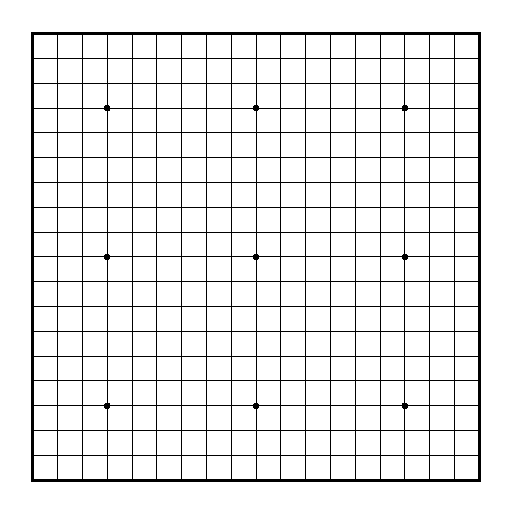
\includegraphics[width=.5\textwidth]{1 - Dia 1}
        \captionsetup{justification=centering}
        \caption*{\emph{Dia.\@~1}}
    \end{center}
    \vspace{-25pt}
\end{wrapfigure}

As pedras são colocadas em containeres chamados de potes. Há dois potes em um conjunto. Um pote é para as pedras pretas, e o outro, para as brancas.

A foto na capa mostra um exemplo de tabuleiro de Go com pernas em um ambiente tradicional japonês. O equipamento de Go pode ser obtido em uma grande gama de qualidade, desde conjuntos muito baratos àqueles custando dezenas de milhares de reais. É possível encontrar uma lista de equipamentos visitando o site da Kiseido: \href{https://www.kiseido.com}{\path{kiseido.com}}~\cite{kiseido}. Na verdade, você nem sequer precisa de um conjunto de Go para estudar ou jogar. É possível simplesmente baixar gratuitamente um programa chamado \emph{Go Write 2} que permite jogar e analisar posições (\href{https://www.gowrite.net/GOWrite2_download.html}{\path{gowrite.net/GOWrite2_download.html}})~\cite{gowrite}. Você também pode jogar partidas online sem custos com oponentes do mundo inteiro, através do servidor KGS (\href{https://www.gokgs.com}{\path{gokgs.com}})~\cite{kgs}. A força dos jogadores lá abrange desde iniciantes até profissionais.

O jogo de Go também pode ser jogado em pequenos tabuleiros, sem nenhuma mudança nas regras, e iniciantes são encorajados a jogar suas primeiras partidas em tabuleiros 9\(\times\)9. Já que uma partida 9\(\times\)9 pode ser finalizada em aproximadamente 10 minutos, esta é uma boa maneira de iniciantes se familiarizarem com as regras e as táticas básicas. Você talvez queira, a partir daí, então jogar algumas partidas em um tabuleiro $13\times13$ antes de progredir para o padrão oficial $19\times19$.
    \chapter{As Regras}\label{chap:regras}

\begin{itemize}
    \item[\textbf{Regra 1}] O tabuleiro começa vazio.
    \item[\textbf{Regra 2}] Preto sempre começa, e, a partir daí, Branco e Preto se alternam. 
    \item[\textbf{Regra 3}] Uma jogada consiste de colocar uma pedra de sua própria cor em uma intersecção vazia do tabuleiro, contanto que tal jogada seja legal, isto é, não conflite com as outras regras.
        
    Os \emph{Diagramas 1 a 3} demonstram uma abertura típica no tabuleiro 9x9. Uma vez jogadas, as pedras permanecem onde estão --- a não ser que capturadas, vide a \emph{Regra 5} ---; elas não podem ser fisicamente movidas para outros pontos. Exceto com pouquíssimas exceções causadas pela \emph{Regra 6}, uma jogada é irrestrita, isto é, você pode jogá-la onde quiser.
    \item[\textbf{Regra 4}] Um jogador pode passar o seu turno a qualquer momento.
    
    Passar geralmente ocorre em somente duas situações:
        
    \begin{enumerate}
        \item Perto do fim da partida;
        \item No início de um partida com pedras de compensação (\emph{handicap}).
    \end{enumerate}
    \item[\textbf{Regra 5}] Uma pedra ou um grupo de uma só cor conectado solidamente é capturado e removido do tabuleiro e mantido como prisioneiro quando todas as suas intersecções diretamente adjacentes são ocupadas pelo inimigo. Os 3 diagramas seguintes demonstram como capturas são executadas.
    \item[\textbf{Regra 6}] Um jogador não pode capturar suas próprias pedras. Ou seja, suicídio é ilegal.
\end{itemize}

\emph{Dia. 4.} Branco ocupa 3 de 4 pontos diretamente adjacentes à pedra preta; isto é, 3 de 4 liberdades. Diz-se que a pedra preta está em atari.

\emph{Dia. 5.} Branco 1 captura a pedra preta através da ocupação de sua última liberdade e a remove do tabuleiro.

\emph{Dia. 6.} Este é o resultado. As pedras capturadas são mantidas separadamente, tipicamente na tampa dos potes, que fica virada do avesso durante a partida.

\emph{Dia. 7 a 9} ilustram a captura na borda do tabuleiro.

\emph{Dia. 10 a 12} ilustram a captura  no canto do tabuleiro.

\emph{Dia. 13 a 15} demonstram  como um grupo de duas pedras solidamente conectado é capturado.

Um grupo solidamente conectado de 5 pedras é capturado nos \emph{Dia. 16 a 18}.

De acordo com a \emph{Regra 6}, é ilegal capturar suas próprias pedras. No \emph{Dia. 19}, as pedras brancas estão em atari. Não é possível salvá-las através da conexão em 1 no \emph{Dia. 20} pois se joga em sua própria liberdade, e as 3 pedras são deixadas sem nenhuma liberdade. Uma jogada assim é ilegal. Em outras palavras, ``a auto-captura é ilegal" ou ``o suicídio é ilegal". Entretanto, se for o turno preto, ele pode capturar as duas pedras brancas jogando em 1 no \emph{Dia. 21}.

A captura das pedras adversárias toma precedência sobre a auto-captura. No \emph{Dia 22}, as duas pedras pretas estão sob atari. Quando Branco 1 é jogado em \emph{Dia 23}, nem não há liberdades para tanto para 1 quanto para as duas pedras pretas à direita, mas são as pedras pretas, não as brancas, que são capturadas. O resultado é mostrado no \emph{Dia 24}. Se Preto quiser capturar, imediatamente, em \textbf{A}, ele pode mas não é obrigatório.

\section{30 Problemas de Captura e Resgate de Pedras}

Aqui estão 30 problemas. Depois de pensar sobre eles, você entenderá completamente como capturar pedras assim como, também, resgatar pedras em risco.

\section{Respostas aos Problemas de 1 a 30}

\begin{itemize}
  \item[\textbf{Resposta ao Problema 1}]
      Preto 1 no \emph{Dia. 1} captura um pedra.

      Se Preto joga 1 no \emph{Dia. 2}, Branco pode resgatar sua pedra através da extensão de 2.
  \item[\textbf{Resposta ao Problema 2}]
      Preto 1 no \emph{Dia. 1} captura uma pedra.

      Se Preto conecta em 1 no \emph{Dia. 2}, Branco pode resgatar sua pedra conectando em 2.
  \item[\textbf{Resposta ao Problema 3}]
      Preto 1 no \emph{Dia. 1} captura uma pedra.

      Se Preto conecta em 1 no \emph{Dia. 2}, Branco pode resgatar sua pedra conectando em 2.
  \item[\textbf{Resposta ao Problema 4}]
      Preto 1 no \emph{Dia. 1} captura duas pedras.

      Se Preto joga 1 no \emph{Dia. 2}, Branco pode resgatar suas pedras estendendo em 2.
  \item[\textbf{Resposta ao Problema 5}]
      Preto 1 no \emph{Dia. 1} captura duas pedras.

      Se Preto estende para 1 no \emph{Dia. 2}, Branco pode resgatar suas pedras conectando em 2.
  \item[\textbf{Resposta ao Problema 6}]
      Preto 1 no \emph{Dia. 1} captura as duas pedras marcadas.

      Se Preto estende para 1 no \emph{Dia. 2}, Branco pode resgatar suas duas pedras capturando as duas pedras pretas com 2.
  \item[\textbf{Resposta ao Problema 7}]
      Preto 1 no \emph{Dia. 1} captura duas pedras.

      Se Preto faz atari com 1 em \emph{Dia. 2}, Branco pode resgatar suas pedras e capturar duas do Preto com 2.
  \item[\textbf{Resposta ao Problema 8}]
      Preto 1 no \emph{Dia. 1} captura duas pedras.

      \emph{Dia. 2} mostra o resultado desta captura.
  \item[\textbf{Resposta ao Problema 9}]
      Preto 1 no \emph{Dia. 1} captura três pedras.

      Se Preto conecta em 1 no \emph{Dia. 2}, Branco pode resgatar sua pedra conectando em 2.
  \item[\textbf{Resposta ao Problema 10}]
      Preto 1 no \emph{Dia. 1} captura três pedras.

      Se Preto joga 1 no \emph{Dia. 2}, Branco pode resgatar as pedras em risco com a conexão em 2.
  \item[\textbf{Resposta ao Problema 11}]
      Preto 1 no \emph{Dia. 1} captura 3 pedras.

      Se Preto joga 1 no \emph{Dia. 2}, Branco pode salvar suas pedras e capturar as 4 pretas com 2.
  \item[\textbf{Resposta ao Problema 12}]
      Preto 1 em \emph{Dia. 1} captura uma pedra (crucial).

      Se Preto estende para 1 no \emph{Dia. 2}, Branco pode resgatar sua pedra conectando em 2.
  \item[\textbf{Resposta ao Problema 13}]
      Preto 1 no \emph{Dia. 1} captura cinco pedras.

      Se Preto joga 1 em \emph{Dia. 2} para escapar do atari, Branco pode resgatar suas cinco pedras conectando em 2.
  \item[\textbf{Resposta ao Problema 14}]
      Preto 1 no \emph{Dia. 1} captura cinco pedras.

      Se Preto conecta em 1 no \emph{Dia. 2}, Branco pode resgatar suas cinco pedras capturando quatro pedras com 2.
  \item[\textbf{Resposta ao Problema 15}]
      Preto pode resgatar sua pedra sob atari conectando em 1 no \emph{Dia. 1}.
      
      Se Preto faz atari com 1 no \emph{Dia. 2}, Branco pode capturar com 2.
  \item[\textbf{Resposta ao Problema 16}]
      Preto 1 no \emph{Dia. 1} resgata sua pedra em atari.

      Se Preto faz atari com 1 no \emph{Dia. 2}, Branco pode capturar uma pedra (crucial) com 2.
  \item[\textbf{Resposta ao Problema 17}]
      Preto 1 no \emph{Dia. 1} salva suas duas pedras sob atari.

      Se Preto faz atari com 1 no \emph{Dia. 2}, Branco pode capturar duas pedras com 2.
  \item[\textbf{Resposta ao Problema 18}]
      Preto 1 no \emph{Dia. 1} resgata sua pedra em atari.

      Se Preto faz atari com 1 no \emph{Dia. 2}, Branco pode capturar uma pedra com 2.
  \item[\textbf{Resposta ao Problema 19}]
      Preto 1 no \emph{Dia. 1} resgata suas três pedras em atari.

      Se Preto faz atari com 1 no \emph{Dia. 2}, Branco pode capturar três pedras com 2.
  \item[\textbf{Resposta ao Problema 21}]
      Preto 1 no \emph{1} resgata suas duas pedras em atari.

      Se Preto faz atari com 1 no \emph{Dia. 2}, Branco captura duas pedras com 2.
  \item[\textbf{Resposta ao Problema 22}]
      Branco não consegue escapar. Se ele rastejar na primeira linha com 1 a 10 no \emph{Dia. 1}, Preto captura oito pedras com 12.

      Após Branco 1 no \emph{Dia 2}, se Preto faz atari a partir da direita com 2, Branco pode escapar com 3 e 5.
  \item[\textbf{Resposta ao Problema 23}]
      Preto precisa fazer atari com 1 no \emph{Dia. 1}. Se Branco 2, Preto captura duas pedras com 3.

      Se Preto faz atari a partir da direita com 1 no \emph{Dia. 2}, ele possui somente uma liberdade, então Branco pode capturar três pedras com 2.
  \item[\textbf{Resposta ao Problema 24}]
      Preto precisa fazer atari com 1 no \emph{Dia. 1}. Se Branco 2, Preto faz atari novamente e suas pedras estão seguras. Se Branco \textbf{A}, Preto captura em \textbf{B}.

      Se Preto faz atari pelo topo com 1 em \emph{Dia. 2}, após Branco 2, as pedras marcadas ficam encarceradas.
  \item[\textbf{Resposta ao Problema 25}]
      Preto precisa fazer atari com 1 no \emph{Dia. 1}. Ele pode agora capturar três pedras com \textbf{A}. Se Branco \textbf{A}, suas pedras ainda estão sob atari.

      Se Preto faz atari com 1 no \emph{Dia. 2}, Branco conecta com 2 e suas pedras escapam.
  \item[\textbf{Resposta ao Problema 26}]
      Se Preto faz atari em 1 no \emph{Dia. 1}, ele captura quatro pedras. Se Branco joga 2, ele não possuirá nenhuma maneira de escapar depois de Preto 3.

      Se Preto faz atari com 1 no \emph{Dia. 2}, Branco estende com 2 e suas pedras escapam.
  \item[\textbf{Resposta ao Problema 27}]
      Preto deveria fazer atari com 1 no \emph{Dia. 1}. Preto pode agora capturar três pedras jogando em \textbf{A}. Se Branco \textbf{A}, suas pedras ainda estão em atari.

      Se Preto faz atari com 1 no \emph{Dia. 2}, Branco conecta com 2 e suas pedras escaparam.
  \item[\textbf{Resposta ao Problema 28}]
      As pedras pretas à direita estão em perigo, então ele precisa fazer atari na pedra marcada com 1 no \emph{Dia. 1}.

      Se Preto faz atari vindo debaixo com 1 no \emph{Dia. 2}, Branco faz atari com 2 e pode capturar em seguida com \textbf{A}.
  \item[\textbf{Resposta ao Problema 29}]
      Preto precisa fazer um duplo-atari  nas pedras marcadas com 1 no \emph{Dia. 1}. Ele pode agora capturar uma pedra em \textbf{A} ou \textbf{B}.

      Preto 1 em \emph{Dia 2} faz atari em somente uma pedra branca. Branco conecta com 2 e Preto não pode capturar nada.
  \item[\textbf{Resposta ao Problema 30}]
      Preto 1 no \emph{Dia. 1} é um duplo-atari, então Branco pode capturar uma das pedras marcadas em \textbf{A} ou \textbf{B}.
      
      Preto 1 no \emph{Dia. 2} faz atari em somente uma pedra. Branco conecta com 2 e Preto não pode capturar nada.
\end{itemize}
    \chapter{A Regra do Ko}

\begin{itemize}
  \item[\textbf{Regra 7}] Nenhuma posição de tabuleiro pode ser recriada.
\end{itemize}

Esta regra requer que todo movimento crie uma nova posição no tabuleiro. Sua principal função é prevenir ciclos infinitos de captura e recaptura em posições de \emph{ko}\footnote{O termo \emph{ko} chegou ao Japão por meio do budismo, vindo da Índia. Em sânscrito, ko aludiria a um ciclo infinito.}, como a exibida no \emph{Dia.\@~25}.

\begin{figure}[h]
  \centering
  \begin{subfigure}[t]{.3\textwidth}
      \centering
      \captionsetup{justification=raggedright,singlelinecheck=false,margin={.05in,.05in}}
      
\includegraphics[width=.9\textwidth]{3 - Dia 25}
      \caption*{\emph{Dia.\@~25. Uma posição de ko}}
  \end{subfigure}
  \hfill
  \begin{subfigure}[t]{.3\textwidth}
      \centering
      \captionsetup{justification=raggedright,singlelinecheck=false,margin={.20in,.05in}}
      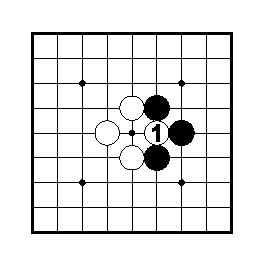
\includegraphics[width=.9\textwidth]{3 - Dia 26}
      \caption*{\emph{Dia.\@~26. Branco captura}}
  \end{subfigure}
  \hfill
  \begin{subfigure}[t]{.3\textwidth}
      \centering
        \captionsetup{justification=centering,singlelinecheck=false,margin={.075in,.05in}}
      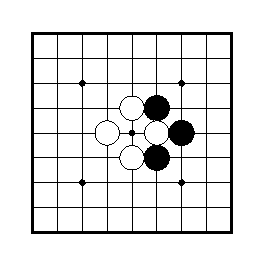
\includegraphics[width=.9\textwidth]{3 - Dia 27}
      \caption*{\emph{Dia.\@~27. Resultado}}
  \end{subfigure}
\end{figure}

Na posição do \emph{Dia.\@~25}, suponha que seja o turno branco. Ele pode capturar uma pedra preta jogando em 1 no \emph{Dia.\@~26}. O resultado é mostrado no \emph{Dia.\@~27}.

Se Preto agora captura com 2 no \emph{Dia.\@~28}\ldots

\pagebreak

\begin{figure}[h]
  \centering
  \begin{subfigure}[t]{.3\textwidth}
      \centering
      \captionsetup{justification=raggedright,singlelinecheck=false,margin={.05in,.05in}}
      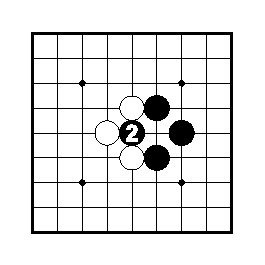
\includegraphics[width=1\textwidth]{3 - Dia 28}
      \caption*{\emph{Dia.\@~28. Uma jogada ilegal}}
  \end{subfigure}
  \hfill
  \begin{subfigure}[t]{.3\textwidth}
      \centering
      \captionsetup{justification=raggedright,singlelinecheck=false,margin={.225in,.05in}}
      
\includegraphics[width=1\textwidth]{3 - Dia 29}
      \caption*{\emph{Dia.\@~29. Mesma posição}}
  \end{subfigure}
  \hfill
  \begin{subfigure}[t]{.3\textwidth}
      \centering
      \captionsetup{justification=raggedright,singlelinecheck=false,margin={.125in,.05in}}
      
\includegraphics[width=1\textwidth]{3 - Dia 30}
      \caption*{\emph{Dia.\@~30. A jogada 3 resolve o ko}}
  \end{subfigure}
\end{figure}

A posição do \emph{Dia.\@~29} é o resultado. Mas, ora, essa é a mesma posição do \emph{Dia.\@~25}. Pela \emph{Regra 7}, isso não é permitido, então Preto precisa jogar em outro lugar. Por exemplo, ele poderia jogar 2 no \emph{Dia.\@~30}. Isso oferece a Branco a oportunidade de conectar em 3, resolvendo o ko.

No \emph{Dia.\@~31}, é o turno Branco a jogar. Uma luta de ko está prestes a acontecer no entorno da pedra preta marcada, que está em atari. O que você acha desta posição? Consegue prever os próximos movimentos? É um grande desafio, tanto em termos de briga de ko como em termos de precisão de jogadas de fim de partida\ldots

\begin{figure}[h]
    \centering
    \captionsetup{justification=centering}
    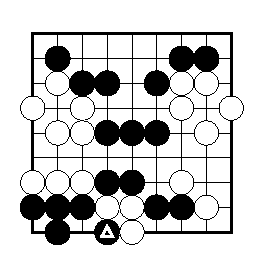
\includegraphics[width=.35\textwidth]{3 - Dia 31}
    \caption*{\emph{Dia.\@~31. Branco a jogar}}
\end{figure}

\pagebreak

Se Branco captura com 1 no \emph{Dia.\@~32}, Preto não pode imediatamente recapturar porque isso reverteria a posição de volta para o \emph{Dia.\@~31}, então ele jogará em outro lugar com Preto 2. Esse tipo de movimento é chamado de \emph{ameaça de ko}.

\begin{figure}[h]
  \centering
  \begin{subfigure}[t]{.3\textwidth}
      \centering
      \captionsetup{justification=raggedright,singlelinecheck=false,margin={.25in,.05in}}
      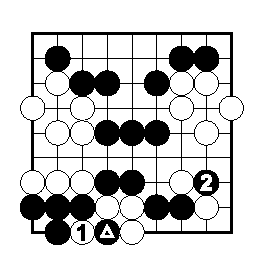
\includegraphics[width=1\textwidth]{3 - Dia 32}
      \caption*{\emph{Dia.\@~32. Uma ameaça de ko}}
  \end{subfigure}
  \hfill
  \begin{subfigure}[t]{.3\textwidth}
      \centering
      \captionsetup{justification=raggedright,singlelinecheck=false,margin={.20in,.05in}}
      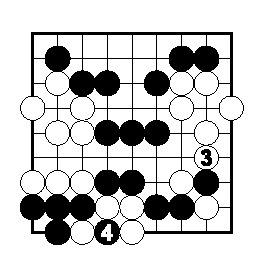
\includegraphics[width=1\textwidth]{3 - Dia 33}
      \caption*{\emph{Dia.\@~33. Branco captura}}
  \end{subfigure}
  \hfill
  \begin{subfigure}[t]{.3\textwidth}
      \centering
      \captionsetup{justification=raggedright,singlelinecheck=false,margin={.05in,.05in}}
      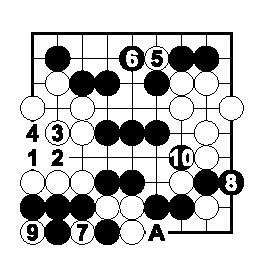
\includegraphics[width=1\textwidth]{3 - Dia 34}
      \caption*{\emph{Dia.\@~34. Resolvendo o ko}}
  \end{subfigure}
\end{figure}

Se Branco responde a essa ameaça com 3 no \emph{Dia.\@~33}, Preto pode recapturar com 4, pois a troca de Preto 2--Branco 3 faz com que a posição global do tabuleiro seja diferente do \emph{Dia.\@~31}. É agora a vez do Branco de encontrar uma ameaça de ko.

Branco corta com 5 no \emph{Dia.\@~34}. Preto poderia ignorar Branco 5 e capturar três pedras em \textbf{A}, e assim  resolver o ko, mas suponhamos que ele responda a Branco 5 com 6. Branco pode agora recapturar o ko com 7. Preto precisa fazer outra ameaça de ko com 8. Talvez Branco ignorará essa ameaça e capturará quatro pedras com 9, finalizando a briga pelo ko. Preto obtém alguma compensação com 10.
    \chapter{O Fim do Jogo}

\begin{itemize}
    \item[\textbf{Regra 8}] Duas passagens de turno consecutivas finalizam a partida. (Ou um dos jogadores pode desistir.)
    \item[\textbf{Regra 9}] No final da partida, toda pedra que não conseguir se salvar é removida do tabuleiro como prisioneira do adversário.
    \item[\textbf{Regra 10}] A pontuação de um jogador é o número de intersecções vazias que ele cercou menos o número de prisioneiros que ele perdeu para o adversário. A pontuação mais alta vence.
\end{itemize}

A partida no \emph{Dia.\@~35} está quase finalizada. Ambos Preto e Branco asseguraram seus respectivos territórios. Durante essa partida, Branco capturou diversos prisioneiros --- indicados pelas sete pedras pretas acima dos diagramas ---, e Preto capturou três pedras brancas.

\begin{figure}[h!]
    \centering
    \begin{subfigure}[t]{.3\textwidth}
        \centering
        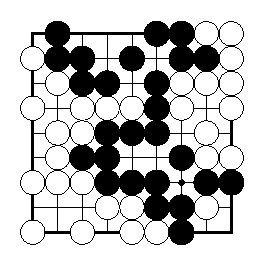
\includegraphics[width=.9\textwidth]{4 - Dia 35}
        \caption*{\emph{Dia.\@~35. Uma ameaça a de ko}}
    \end{subfigure}
    \hfill
    \begin{subfigure}[t]{.3\textwidth}
        \centering
        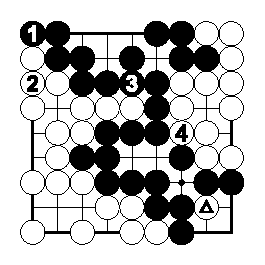
\includegraphics[width=.9\textwidth]{4 - Dia 36}
        \caption*{\emph{Dia.\@~36. Branco captura}}
    \end{subfigure}
    \hfill
    \begin{subfigure}[t]{.3\textwidth}
        \centering
        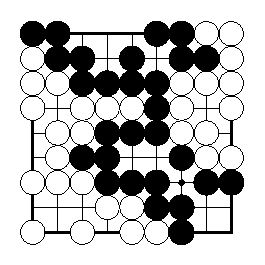
\includegraphics[width=.9\textwidth]{4 - Dia 37}
        \caption*{\emph{Dia.\@~37. Resolvendo o ko}}
    \end{subfigure}
    \caption*{\emph{Como capturas, Preto possui três pedras, e Branco, sete.}}
\end{figure}
  
Preto 1 no \emph{Dia.\@~36} não conquista nenhum ponto, mas ameaça a captura de uma pedra branca e o início de um ko, então Branco conecta com 2. Preto 3 e Branco 4 não ganham pontos também. Há pontos neutros que são jogados ao final da partida, somente para mais claramente delimitar os territórios. Não há mais pontos a serem disputados, então Preto 5 e Branco 6 são passagens de turno. De acordo com a \emph{Regra 8}, isso finaliza a partida.

A pedra branca marcada no \emph{Dia.\@~36} está morta: ela não consegue evitar de ser capturada. Portanto, de acordo com a \emph{Regra 9}, ela é removida do tabuleiro como prisioneira. O resultado dessa operação é visualizado no \emph{Dia.\@~37}. Note que Preto possui quatro prisioneiros brancos.

Vamos contar a pontuação.

\begin{figure}[h!]
    \centering
    \begin{subfigure}[t]{.3\textwidth}
        \centering
        
\includegraphics[width=.9\textwidth]{4 - Dia 38}
        \caption*{\emph{Dia.\@~38. O território preto}}
    \end{subfigure}
    \hfill
    \begin{subfigure}[t]{.3\textwidth}
        \centering
        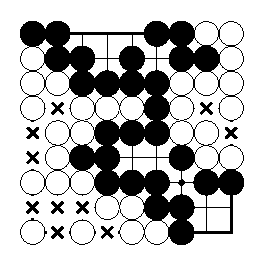
\includegraphics[width=.9\textwidth]{4 - Dia 39}
        \caption*{\emph{Dia.\@~39. O território branco}}
    \end{subfigure}
    \hfill
    \begin{subfigure}[t]{.3\textwidth}
        \centering
        
\includegraphics[width=.9\textwidth]{4 - Dia 40}
        \caption*{\emph{Dia.\@~40. O território é preenchido com prisioneiros}}
    \end{subfigure}
    \caption*{\emph{Como capturas, Preto possui três pedras, e Branco, sete.}}
\end{figure}

Preto cercou os pontos vazios marcados com \textbf{X} no \emph{Dia.\@~38}, e Branco cercou os pontos vazios marcados com \textbf{X} no \emph{Dia.\@~39}. Esses pontos vazios cercados são denominados de \emph{território}.

Para subtrair prisioneiros do território, os prisioneiros são colocados no tabuleiro dentro dos territórios pretos e brancos, como mostrado pelas pedras marcadas no \emph{Dia.\@~40}. Conte os territórios para cada lado e verá que Branco possui 6 pontos enquanto que Preto possui 5 pontos. Branco vence por um ponto.

Essas são as dez regras necessárias para se jogar Go. Há algumas poucas posições especiais e kos que são determinados por adjudicação. Essas posições são conhecidas como Precedentes da Nihon Kiin, mas elas ocorrem muito raramente em partidas.

As regras aqui apresentadas são as japonesas. Há outras também, a mais importante dentre essas outras sendo as regras chinesas. A maioria dos jogadores no ocidente utilizam as regras japonesas. Porém, se você for jogar Go na China, você terá de aprender sobre as regras chinesas. A principal diferença entre elas é o procedimento de contagem ao final da partida, mas, para basicamente todos os fins práticos, ambas são equivalentes. Isto é, elas não mudam a natureza do jogo. Para uma exposição dos diversos conjuntos de regras, assim como os Precedentes da Nihon Kiin, veja o livro \emph{The Go Player's Almanac}~\cite{bozulich_almanac}.
    \chapter{Partidas-Exemplo}\label{chap:cinco}

\section{Partida-Exemplo em um Tabuleiro \texorpdfstring{6$\times$6}{6x6}}

A partida a seguir ilustra jogadas perfeitas em um tabuleiro 6x6, o menor tamanho que Go é interessante de ser jogado.

\emph{Dia.\@~1} Isso pode ser chamado de abertura. Preto começa por tentar controlar o lado direito com 1 e 3, e Branco, controle do lado esquerdo com 2 e 4. Preto se dobra em volta de Branco com 5 e 7, e Branco resiste com 6 e 8.

\begin{figure}[h!]
  \centering
  \begin{subfigure}[t]{.3\textwidth}
      \centering
      
\includegraphics[width=.9\textwidth]{5 - Dia 1}
      \caption*{\emph{Dia.\@~1. (1-8)}}
  \end{subfigure}
  \hfill
  \begin{subfigure}[t]{.3\textwidth}
      \centering
      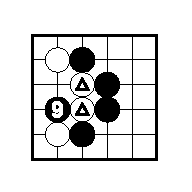
\includegraphics[width=.9\textwidth]{5 - Dia 2}
      \caption*{\emph{Dia.\@~2. (9)}}
  \end{subfigure}
  \hfill
  \begin{subfigure}[t]{.3\textwidth}
      \centering
      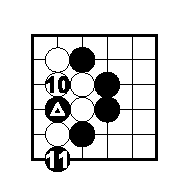
\includegraphics[width=.9\textwidth]{5 - Dia 3}
      \caption*{\emph{Dia.\@~3. (10-11)}}
  \end{subfigure}
\end{figure}

\emph{Dia.\@~2} Preto pressiona sua vantagem através do corte em 9. Isso põe as duas pedras marcadas em atari --- as pedras pretas estão ocupando todas as liberdades brancas exceto uma. Note que as pedras brancas marcadas não estão diretamente conectadas às outras pedras brancas.

\emph{Dia.\@~3} Branco resgata suas duas pedras pela conexão com 10, e a pedra preta marcada agora está em atari. Preto ignora isso e joga 11, colocando a pedra branca em atari.

\pagebreak

\emph{Dia.\@~4} Branco escapa do atari descendo para 12. Preto conecta com 13 para prevenir que Branco corte ali. A pedra preta marcada ainda está sob atari. Entretanto, ela não pode escapar, então Branco não se importa em capturá-la e corta em 14, colocando outra pedra preta em atari.

\begin{figure}[h!]
  \centering
  \begin{subfigure}[t]{.3\textwidth}
      \centering
      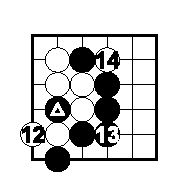
\includegraphics[width=.9\textwidth]{5 - Dia 4}
      \caption*{\emph{Dia.\@~4. (12-14)}}
  \end{subfigure}
  \hfill
  \begin{subfigure}[t]{.3\textwidth}
      \centering
      
\includegraphics[width=.9\textwidth]{5 - Dia 5}
      \caption*{\emph{Dia.\@~5. (15-18)}}
  \end{subfigure}
  \hfill
  \begin{subfigure}[t]{.3\textwidth}
      \centering
      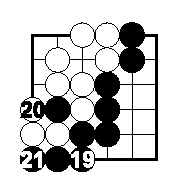
\includegraphics[width=.9\textwidth]{5 - Dia 6}
      \caption*{\emph{Dia.\@~6. (19-21)}}
  \end{subfigure}
\end{figure}

\emph{Dia.\@~5} Preto joga um atari com 15 e Branco captura com 16, tomando um prisioneiro. Preto agora desce para 17, ameaçando jogar em 18 e desprivilegiar Branco de um ponto. Sendo assim, Branco precisa conectar em 18. Esse é o último movimento da partida e vale um ponto.

\emph{Dia.\@~6} Preto conecta com 19, preparando para tomar o último ponto neutro em 21. Branco não pode jogar em 21, então ele captura com 20, tomando outro prisioneiro.

\emph{Dia.\@~7} Após Preto 21 no \emph{Dia.\@~6}, não há mais pontos a serem ganhos ou disputados, então Branco passa. Preto também passa. De acordo com a \emph{Regra 8}, o jogo termina.

\begin{figure}[h!]
  \centering
  \begin{subfigure}[t]{.3\textwidth}
      \centering
      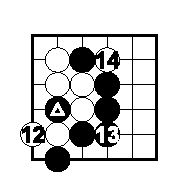
\includegraphics[width=.9\textwidth]{5 - Dia 4}
      \caption*{\emph{Dia.\@~7. Partida finalizada}}
  \end{subfigure}
  \hspace{1cm}
  \begin{subfigure}[t]{.3\textwidth}
      \centering
      
\includegraphics[width=.9\textwidth]{5 - Dia 5}
      \caption*{\emph{Dia.\@~8}}
  \end{subfigure}
\end{figure}

\emph{Dia.\@~8} Branco possui dois prisioneiros, então ele os coloca no território preto --- as duas pedras marcadas. Os territórios são agora contados. Branco possui 6 pontos, e Preto, 9.

\textbf{Preto vence por 3 pontos.}

\pagebreak

\section{Perguntas e Respostas}

\begin{itemize}
    \item[\textbf{Pergunta}]
      Ao invés de 19 no \emph{Dia.\@~6}, será que Preto não poderia jogar atari em 2?
    \item[\textbf{Resposta}] 
      Se Preto fizer atari imediatamente com 1 em \emph{Dia.\@~9}, ele se colocaria em atari e perderia  duas pedras após a captura Branca com 2.

    \begin{figure}[h!]
      \centering
      \begin{subfigure}[t]{.3\textwidth}
          \centering
          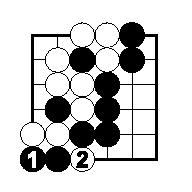
\includegraphics[width=.9\textwidth]{5 - Dia 9}
          \caption*{\emph{Dia.\@~9}}
      \end{subfigure}
      \hspace{1cm}
      \begin{subfigure}[t]{.3\textwidth}
          \centering
          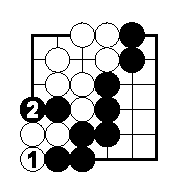
\includegraphics[width=.9\textwidth]{5 - Dia 10}
          \caption*{\emph{Dia.\@~10}}
      \end{subfigure}
    \end{figure}

    \item[\textbf{Pergunta}]
      Ao invés de capturar com 20 no \emph{Dia.\@~6}, será que Branco não poderia jogar no último ponto neutro em 21?
    \item[\textbf{Resposta}] 
      Se Branco jogar imediatamente em 1 no \emph{Dia.\@~10}, ele colocaria três de suas pedras em atari, e Preto procederia com a captura em 2.
    \item[\textbf{Pergunta}]
      Por que Branco passou no \emph{Dia.\@~7}? Por que ele não tenta invadir o território com 1 no \emph{Dia.\@~11}?
    \item[\textbf{Resposta}] 
      Não há regra que previna Branco de invadir. Mas ele percebe que seria de nenhuma utilidade. Preto responderia com 2 no \emph{Dia.\@~12}, colocando a pedra invasora em atari, e, quando Preto captura com 6, Branco perderia sua força invasora completamente.

    \begin{figure}[h!]
      \centering
      \begin{subfigure}[t]{.3\textwidth}
          \centering
          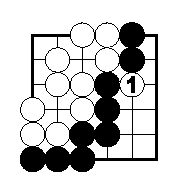
\includegraphics[width=.9\textwidth]{5 - Dia 11}
          \caption*{\emph{Dia.\@~11}}
      \end{subfigure}
      \hspace{1cm}
      \begin{subfigure}[t]{.3\textwidth}
          \centering
          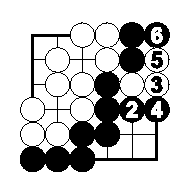
\includegraphics[width=.9\textwidth]{5 - Dia 12}
          \caption*{\emph{Dia.\@~12}}
      \end{subfigure}
    \end{figure}

    \item[\textbf{Pergunta}]
      Se Branco continuar insistindo na invasão, ele não conseguirá, no final, ocupar todos os pontos dentro do grupo Preto e, assim, capturá-lo?

    \begin{figure}[h!]
      \centering
      \begin{subfigure}[t]{.3\textwidth}
          \centering
          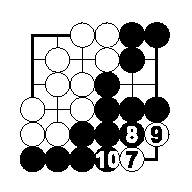
\includegraphics[width=.9\textwidth]{5 - Dia 13}
          \caption*{\emph{Dia.\@~13}}
      \end{subfigure}
      \hfill
      \begin{subfigure}[t]{.3\textwidth}
          \centering
          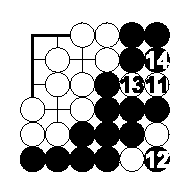
\includegraphics[width=.9\textwidth]{5 - Dia 14}
          \caption*{\emph{Dia.\@~14}}
      \end{subfigure}
      \hfill
      \begin{subfigure}[t]{.3\textwidth}
        \centering
        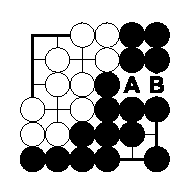
\includegraphics[width=.9\textwidth]{5 - Dia 15}
        \caption*{\emph{Dia.\@~15}}
      \end{subfigure}
    \end{figure}

    \item[\textbf{Resposta}] 
      Ele é bem-vindo para tentar, como no \emph{Dia.\@~13}, mas ele não será bem sucedido. Após Branco 7 e 9, Preto esmaga aquelas duas pedras com 10 --- Branco não pode conectar no ponto 1-1, já que seria suicídio, um movimento ilegal. Branco põe o grupo preto de 11 pedras em atari com 11 no \emph{Dia.\@~14} e Preto captura duas pedras com 14. No final, Branco esgota os possíveis pontos de invasão. A posição agora aparenta ser \emph{Dia.\@~15} e Preto ainda vence por 3 pontos. Lembre-se que as pedras brancas voltarão para o território Branco quando a partida for contabilizada. Branco pode tentar novamente em \textbf{A}, mas Preto capturará imediatamente com \textbf{B}.
      
      O que faz com que o grupo preto inteiro no \emph{Dia.\@~15} seja invulnerável à captura são os vários buracos, ou olhos, que ele possui. Branco pode jogar somente uma pedra por vez, portanto ele jamais conseguirá preencher todos esses olhos simultaneamente, sem se suicidar, como ele deveria, para capturar o grupo preto.
    \item[\textbf{Pergunta}]
      Quantos olhos são necessários para que um grupo esteja seguro?
    \item[\textbf{Resposta}] 
      Ele precisa de dois, pelo menos. \emph{Dia.\@~16} mostra dois exemplos. Os dois grupos pretos estão vivos com dois olhos cada um. Na verdade, Branco não possui um movimento legal para atacar também. Branco, com seus dois grandes espaços de olhos, também está vivo. Preto pode jogar dentro do grupo branco, mas Branco pode facilmente capturar os invasores.

      \begin{figure}[h!]
        \centering
        \begin{subfigure}[t]{.3\textwidth}
            \centering
            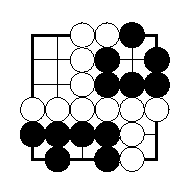
\includegraphics[width=.9\textwidth]{5 - Dia 16}
            \caption*{\emph{Dia.\@~16}}
        \end{subfigure}
        \hfill
        \begin{subfigure}[t]{.3\textwidth}
            \centering
            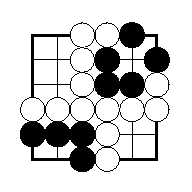
\includegraphics[width=.9\textwidth]{5 - Dia 17}
            \caption*{\emph{Dia.\@~17}}
        \end{subfigure}
        \hfill
        \begin{subfigure}[t]{.3\textwidth}
          \centering
          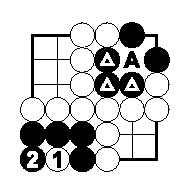
\includegraphics[width=.9\textwidth]{5 - Dia 18}
          \caption*{\emph{Dia.\@~18 Branco 3 em 1}}
        \end{subfigure}
      \end{figure}

      Você deveria também notar que os olhos precisam estar separados. O grupo preto no canto inferior esquerdo no \emph{Dia.\@~17} não está vivo, mas morto. Ele não consegue evitar de ser capturado. Talvez possa parecer que ele possui dois olhos, mas estes não separáveis ou distintos. Branco 1 no \emph{Dia.\@~18} coloca Preto em atari. Preto pode capturar com 2, mas Branco só joga novamente em 1 com 3, privando o grupo preto de sua última liberdade e, assim, capturando todas as cinco pedras pretas.

      Outra coisa sobre a qual se atentar é olho falso, como o que o grupo preto possui no canto superior direito do \emph{Dia.\@~18} em \textbf{A}. Esse grupo também está morto. Branco \textbf{A} captura as três pedras marcadas e põe as outras duas pedras sob atari.
    \item[\textbf{Pergunta}]
      Um grupo sempre precisa estar apto a criar dois olhos para estar vivo?

      \begin{figure}[h!]
        \centering
        \begin{subfigure}[t]{.3\textwidth}
            \centering
            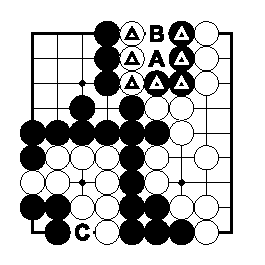
\includegraphics[width=.9\textwidth]{5 - Dia 19}
            \caption*{\emph{Dia.\@~19}}
        \end{subfigure}
      \end{figure}
    \item[\textbf{Resposta}] 
      Geralmente, mas há exceções. No \emph{Dia.\@~19}, o grupo preto marcado e o grupo branco não possuem nenhum olho, mas ambos compartilham liberdades. Nenhum dos lados pode atacar o outro jogando \textbf{A} ou \textbf{B} sem se colocar em atari, então nenhum dos lados deveria jogar nessa região, ou seja, ambos os grupos estão vivos. Este tipo de impasse local é chamado de \emph{seki}. Os pontos vazios entre as pedras marcadas não contam como território para nenhum dos lados.

      Há outro seki no canto inferior esquerdo do \emph{Dia.\@~19}. O grupo preto de três pedras e o grupo branco cercando-o ambos possuem um olho só e nenhum deles pode ocupar o ponto \textbf{C} entre eles sem se colocar sob atari. (O ponto \textbf{C} também não é território.)
\end{itemize}

\pagebreak

\section{Partida-Exemplo em um Tabuleiro \texorpdfstring{9$\times$9}{9x9}}

\emph{Dia.\@~1} A boa estratégia dita que movimentos de abertura sejam feitos na terceira linha ou acima, em relação às bordas do tabuleiro. Nesse caso, Preto 1 e Branco 2 são jogados nas quartas linhas.

\begin{figure}[h!]
  \centering
  \begin{subfigure}[t]{.3\textwidth}
      \centering
      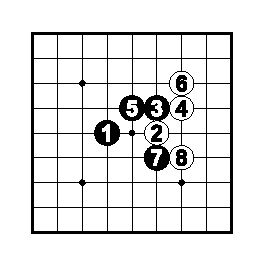
\includegraphics[width=.9\textwidth]{5 - Game 2 - Dia 1}
      \caption*{\emph{Dia.\@~1 (1-8)}}
  \end{subfigure}
  \hfill
  \begin{subfigure}[t]{.3\textwidth}
      \centering
      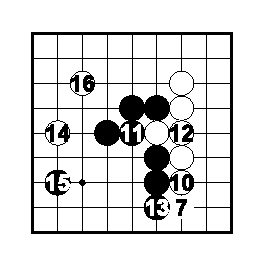
\includegraphics[width=.9\textwidth]{5 - Game 2 - Dia 2}
      \caption*{\emph{Dia.\@~2 (9-16)}}
  \end{subfigure}
  \hfill
  \begin{subfigure}[t]{.3\textwidth}
    \centering
    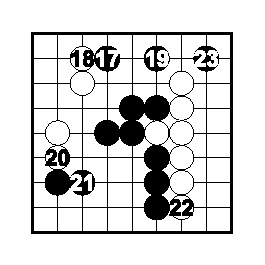
\includegraphics[width=.9\textwidth]{5 - Game 2 - Dia 3}
    \caption*{\emph{Dia.\@~3 (17-23)}}
  \end{subfigure}
\end{figure}

\emph{Dia.\@~2} Preto 11 faz atari na pedra branca, então Branco conecta em 12. Tendo construído um grupo vivo à direita, Branco invade o lado esquerdo com 14 e inicia a construção de outro grupo vivo à esquerda com 16.

\emph{Dia.\@~3} Branco defende seu grupo no lado esquerdo com 18 e 20, e, então, seu grupo à direita com 22. Preto pula para o lado direito com 23 e o fim de jogo se inicia. Pulos de um espaço como 19 e 23 são frequentemente boas jogadas.

\emph{Dia.\@~4} Branco detém a intrusão preta ao lado esquerdo com 24 e 26. As jogadas começam, a partir de agora, a focar nas bordas do tabuleiro.

\begin{figure}[h!]
  \centering
  \begin{subfigure}[t]{.3\textwidth}
      \centering
      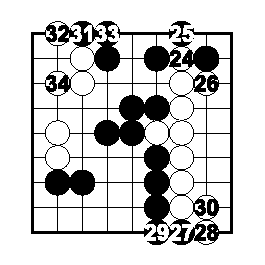
\includegraphics[width=.9\textwidth]{5 - Game 2 - Dia 4}
      \caption*{\emph{Dia.\@~4 (24-34)}}
  \end{subfigure}
  \hspace{1cm}
  \begin{subfigure}[t]{.3\textwidth}
      \centering
      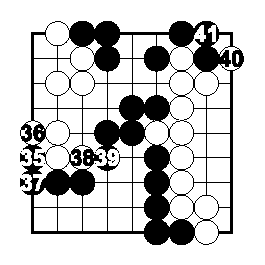
\includegraphics[width=.9\textwidth]{5 - Game 2 - Dia 5}
      \caption*{\emph{Dia.\@~5 (35-41)}}
  \end{subfigure}
\end{figure}

\emph{Dia.\@~5} O fim de jogo continua com Preto 35 até o atari de Branco 40.

\pagebreak

\emph{Dia.\@~6} Branco 50 é um sacrifício que, mais tarde, forçará Preto a conectar em 55. No final da partida, Branco perdeu um prisioneiro --- a pedra em 50 --- e Preto 53 é uma pedra morta.

\begin{figure}[h!]
  \centering
  \begin{subfigure}[t]{.3\textwidth}
      \centering
      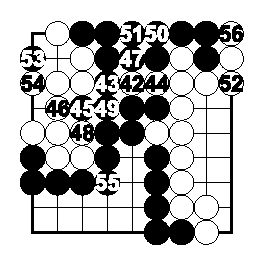
\includegraphics[width=.9\textwidth]{5 - Game 2 - Dia 6}
      \caption*{\emph{Dia.\@~6 (42-57)}}
  \end{subfigure}
  \hfill
  \begin{subfigure}[t]{.3\textwidth}
      \centering
      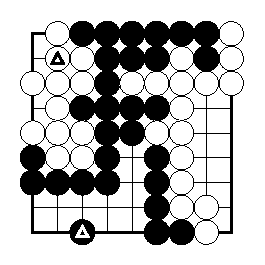
\includegraphics[width=.9\textwidth]{5 - Game 2 - Dia 7}
      \caption*{\emph{Dia.\@~2 Prisioneiros}}
  \end{subfigure}
  \hfill
  \begin{subfigure}[t]{.3\textwidth}
    \centering
    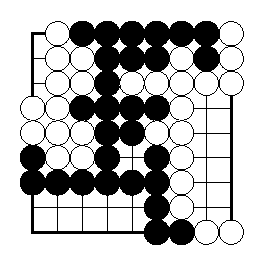
\includegraphics[width=.9\textwidth]{5 - Game 2 - Dia 8}
    \caption*{\emph{Dia.\@~8 Rearranjo}}
  \end{subfigure}
\end{figure}

\emph{Dia.\@~7} O prisioneiro branco é substituído dentro do território Branco, e a pedra preta morta --- 53 no \emph{Dia.\@~6} --- é removida e preenche o interior do território preto. Essas pedras são indicadas pelas pedras marcadas.

\emph{Dia.\@~8} É costumeiro rearranjar os territórios durante a contagem mais facilmente reconhecível em termos de múltiplos de 10. Nesta partida, Preto possui 11 pontos de território, e Branco, 13, portanto, Branco vence por dois pontos.
    \chapter{Estratégia de Abertura}\label{chap:6:estrat_abertura}

Para se tornar um jogador forte de Go, é necessário desenvolver duas habilidades:

\begin{enumerate}
    \item a habilidade de ler à frente movimento por movimento e prever os resultados de embates locais;
    \item a habilidade de intuir o que está acontecendo no tabuleiro como um todo.
\end{enumerate}

O balanço aproximadamente igualitário entre qualidades intuitivas e analíticas é grande parte da atratividade do Go. Na abertura, quando o tabuleiro consiste de majoritariamente espaço vazio, é intuição, e uma base de dados de conhecimento geral, que toma um papel dominante.

No tabuleiro $19\times19$, o tamanho oficial, é difícil de se assegurar território no início, então a partida usualmente começa com os jogadores espaçando suas pedras para formar grandes armações dentro das quais eles poderão brigar vantajosamente no futuro.

\emph{Dia. 1 a 3} mostra uma abertura típica no tabuleiro $19\times19$.

É geralmente muito mais fácil de se estabelecer bases nos cantos, como Preto e Branco o fazem com 1 a 4 no \emph{Dia. 1}. Uma ou duas pedras por canto é suficiente. Com 5, Preto estabelece um enclausuro de canto. Esse movimento delimita e vigia o território no canto. Não é ainda território seguro, uma vez que Branco possui múltiplas maneiras de invadi-lo. Mas Preto terá a vantagem em qualquer luta que se irromper ali. O tempo para a invasão branca será, assim, um fator crítico.

Aproximar-se do canto com Branco 6 no \emph{Dia. 2}, onde Preto possui somente uma pedra, é uma boa jogada. Isso frequentemente provoca lutas, como o curto conflito que se segue. Nos movimentos de 7 a 12, Preto assegura  o canto enquanto Branco constrói uma posição à direita. Essa sequência é um dos padrões-referência conhecidos como josekis.

Preto 13 no \emph{Dia. 13} é outro exemplo de outra aproximação. Branco 14 forma uma armação esparsa no canto inferior esquerdo do tabuleiro a partir da pedra branca marcada. A terceira ou a quarta linha é a melhor para extensões como esta. Preto desenvolve uma armação no topo com 15 e 17. Note Preto 17 na quarta linha, e Preto 15 e a pedra preta marcada na terceira linha. Isso constitui um balanço ideal de jogadas altas e baixas. As pedras na terceira linha defendem os flancos da posição preta enquanto que a pedra na quarta linha expande seu território para o centro.

\section{A Primeira Prioridade: Estabelecer uma Presença no Canto}

A abertura de uma partida de Go geralmente se inicia com ambos os lados estabelecendo presenças nos cantos. Os pontos a seguir são os cinco de referência que um jogador usualmente ocupa com seus primeiros movimentos.

\emph{Dia. 1. O ponto 3-3.} O intuito de Preto 1 no ponto 3-3 --- também conhecido como \emph{san-san} --- é assegurar o território no canto, apesar de que esse movimento não fornece muita influência no centro.

\emph{Dia. 2. O ponto-estrela.} Por ter jogado no ponto 4-4 --- também conhecido como ponto-estrela --- com 1, Preto almeja influência no centro.

\emph{Dia. 3. O ponto 3-4.} Quando Preto joga 1 no ponto 3-4 (\emph{komoku}), ele espera ganhar território ao longo do lado direito assim como algo no canto.

\emph{Dia. 4. O ponto 5-3.} Preto 1 no ponto 5-3 (\emph{mokuhazushi}) enfatiza o lado. Preto está disposto a conceder a maior parte do canto para Branco.

\emph{Dia. 5. O ponto 5-4.} Preto 1 no ponto 5-4 (\emph{takamoku}) concede o canto ao Branco. Ele almeja influência no centro e ao longo dos lados.

\section{Movimentos de Aproximação}

Depois de os jogadores terem ocupado os cantos, é praxe atacá-los ou desafiá-los. Tais movimentos são conhecidos como movimentos de aproximação.

Uma pedra no 3-3 vai geralmente ser atacada por um movimento no ponto 4-4 --- Branco 1 no \emph{Dia. 6}. Com movimentos até Branco 7, Preto assegura o território no canto, mas Branco ganha influência no centro. Essa sequência é um padrão estabelecido como joseki. Seria uma boa ideia memorizar esse padrão básico e outros conforme continuamos, uma vez que eles são alguns dos mais comuns que você encontrará.

Contra uma pedra jogada no ponto 4-4, é usual se aproximar com um movimento do cavaleiro --- similar ao do cavalo no xadrez --- de Branco 1 no \emph{Dia. 7}. Preto 2 é a resposta típica, mas Preto 2 em \textbf{A} ou \textbf{B} também são frequentemente jogados. Branco agora continua deslizando para 3, Preto defende o canto com 4, e Branco estende dois espaços até 5. Isso também é um joseki básico.

Ao invés de 1 no \emph{Dia. 7}, Branco poderia também invadir o ponto 3-3 com 1 no \emph{Dia. 8}. A sequência até Preto 12 é outro joseki básico. Branco consegue um território blindado no canto, mas Preto obtém uma posição muito densa no exterior. Se não houver muitas pedras no tabuleiro, a densidade preta é julgada como melhor do que o território branco, portanto não é aconselhável que Branco jogue essa sequência até que o meio de jogo comece. Esse joseki enfatiza a principal fraqueza da pedra situada no ponto 4-4: ela deixa o canto aberto para invasões. No entanto, um jogador que queira prosseguir com uma estratégia que enfatize influência central vai geralmente jogar uma pedra ou no ponto 4-4 ou no ponto 5-4.

Contra uma pedra no ponto 3-4, há duas aproximações básicas: o movimento curto do cavaleiro em \textbf{A} no \emph{Dia. 9} e a aproximação de um espaço em \textbf{B}.

Contra a aproximação curta do cavaleiro de Branco 1 no \emph{Dia. 10}, Preto 2 é uma resposta sólida. Branco pode responder estendendo até 3 ou mesmo tão distantemente quanto \textbf{A}.

Se Branco joga a aproximação de um espaço de 1 no \emph{Dia. 11}, contatar-se com Preto 2 é uma resposta popular. A sequência até Branco 7 é um joseki básico. Preto assegura o canto e Branco estabelece uma posição no topo. Preto poderia também jogar 6 em \textbf{A}, e Branco poderia jogar 7 em \textbf{B}. Compare esse joseki a movimentos como 6 a 12 no \emph{Dia. 2} no início desta seção sobre estratégia de abertura.

Quando Preto possui uma pedra no ponto 5-3 (a pedra marcada), Branco 1 no \emph{Dia. 12} é a aproximação padrão. Preto responde achatando Branco com 2 e 4. Branco assegura o território à direita com 3 e 5 e Preto estende a partir de sua parede com 6, estabelecendo uma posição no topo.

O intuito de se jogar uma pedra preta no ponto 5-4 (a pedra marcada) no \emph{Dia. 13} é ganhar influência no centro. Quando Branco se aproxima com 1, Preto joga 2, confinando Branco ao canto. Com a sequência até 7, Branco garante o território no canto, e Preto ganha a influência no centro.

\section{Pinças}

Quando um lado faz um movimento de aproximação, o outro frequentemente segue com uma pinça.

Após Branco se aproximar com a pedra no 4-4 com 1 no \emph{Dia. 14}, Branco pode jogar uma pinça com 2. (Pinças de \textbf{A} a \textbf{E} também são possíveis e frequentemente jogadas.) Em resposta, Branco geralmente invade o canto com 3 no \emph{Dia. 15}. A sequência até Branco 11 é um joseki. Branco ganha território no canto, e Preto consegue uma posição densa no entorno.

Quando Preto possui a pedra marcada, como no \emph{Dia. 16}, a direção correta para Preto bloquear é por baixo com 4. Os movimentos até Preto 8 também constituem um joseki. Novamente, Branco consegue o canto, mas Preto conseguiu mapear uma armação territorial no lado superior direito com sua parede e a pedra marcada.

Se Branco não estiver satisfeito com o resultado no \emph{Dia. 16}, em que Preto possui uma presença esmagadora no centro enquanto que suas próprias pedras se confinam ao canto, ele pode optar pela resposta 3 à Preto 2 no \emph{Dia. 17}. Após a sequência joseki até 13, Preto assegurou uma posição no topo e, ainda, mapeou uma esfera de influência no lado direito, mas Branco conseguiu estabelecer uma presença no centro. Branco 13 em \textbf{A} também é uma jogada tida como joseki.

No \emph{Dia. 18}, Branco se aproxima da pedra marcada no ponto 3-4 com 1, e Preto joga a pinça com 2. Branco sai para o centro com o movimento diagonal de 3, e Preto defende o lado direito com 4. Finalmente, Branco estabelece uma base para suas pedras deslizando até 5, e Preto delimita seu território no lado direito com a extensão até 6.

Apesar de que um pouco distante, Preto 2 no \emph{Dia. 19} é também uma pinça contra 1. Branco sai para o centro com seu pulo de dois espaços em 3. Preto defende o lado direito com 4, e Branco faz uma base com suas pedras de 5 a 9.

Preto 2 no \emph{Dia. 19} é o mais distante que uma pedra pode ser jogada para ser denominada como pinça. Por exemplo, Preto 2 no \emph{Dia. 20} não é uma pinça contra a pedra branca em 1 pois Branco pode jogar a extensão ideal de 3.

Contra a aproximação alta de Branco 1 no \emph{Dia. 21}, há diversas pinças que podem ser jogadas. Preto 2, \textbf{A} e \textbf{B} são as mais comuns. Se Branco responder Preto 2 pulando ao centro com 3, Preto defenderá de maneira disciplinada e apertada o lado direito com 4.

\section{Josekis}

Nas seções sobre aproximações e pinças, vários josekis básicos foram introduzidos. Esses josekis são tão básicos que eles constantemente surgem em partidas, então é uma boa ideia memorizá-los. Josekis provêm exemplos de bons movimentos que você pode aplicar a posições em seus próprios jogos, sendo assim, ao estudá-los, você gradativamente afiará sua intuição sobre o que constitui uma boa jogada.

Um bom livro para se começar a estudar josekis é \emph{38 Basic Josekis}~\cite{kosugi_bozulich_38_basic_joseki}. Conforme você se tornar mais forte, você irá querer um livro de referência mais completo no assunto. Para esse propósito, nós recomendamos a coleção de dois volumes \emph{21st Century Dictionary of Basic Josekis}~\cite{takao_shinji_21st_century_joseki_dictionary}, por Takao Shinji 9p. Apesar de que ele não contém algumas inovações recentes, outro excelente livro é o livro \emph{A Dictionary of Basic Josekis}~\cite{ishida_yoshio_basic_joseki_dictionary}, por Ishida Yoshio 9p. Ele contém muitos exemplos de jogos nos quais os josekis foram estudados e utilizados. Todos esses livros foram publicados pela Kiseido~\cite{kiseido}.

\section{Enclausuros de Canto}

Ao invés de fazer uma jogada de aproximação, um jogador talvez escolha reforçar uma pedra que ele já jogou em um canto, com um enclausuro. Na abertura mostrada no \emph{Dia. 22}, após Branco 4, Preto faz um enclausuro de movimento de cavaleiro curto com com 5. Preto poderia também fazer o enclausuro de um espaço jogando em \textbf{A} ou o de cavaleiro longo com \textbf{B}. Essas são todas boas jogadas, mas o de cavaleiro curto é o que mais vem sendo jogado ultimamente pois tende a melhor defender o canto. O enclausuro de um espaço de Branco 6 é jogado para enfatizar o centro, mas, já que possui um flanco aberto, está vulnerável a um ataque ao redor de \textbf{C}.

\section{Extensões}

Até aqui, consideramos movimentos feitos primariamente em torno do canto. Conforme a partida progride, extensões ao longo dos lados precisarão ser feitas. Extensões precisam trabalhar eficientemente. Elas deveriam não ser demasiado curtas nem demasiado longas. Há três princípios relacionados que oferecem diretivas para a criação de extensões eficientes.

\begin{itemize}
    \item[\textbf{Princípio 1}] De uma pedra só, estenda dois espaços.
        
        De uma pedra só na terceira linha, uma extensão de dois espaços é a mais eficiente. Por exemplo, Branco faz um aproximação de cavaleiro longo contra a pedra preta no ponto 3-4 com 1 no \emph{Dia. 23}. Se Preto defende o canto com 2, a extensão de dois espaços de Branco 3 é a resposta ideal. Isso é um joseki e possui a distinção de ser um dos mais curtos. (Outro joseki curto é mostrado no \emph{Dia. 10}.) 
    \item[\textbf{Princípio 2}] De uma parede de duas pedras, estenda três espaços.
    
        No \emph{Dia. 24}, Branco possui uma parede de duas pedras (as pedras marcadas). A partir dessa parede, estender três espaço para 1 é o ideal. (Essa posição foi gerada a partir do joseki mostrado no \emph{Dia. 11}, apesar de que em uma orientação diferente.)
    \item[\textbf{Princípio 3}] De uma parede de três pedras, estenda quatro espaços. 

        No \emph{Dia. 25}, Branco fez uma parede de três pedras (as pedras marcadas), então ele pode estender quatro espaços até 1.
\end{itemize}

Esses princípios não são tão rígidos; eles deveriam ser interpretados como diretivas. Suas extensões precisam trabalhar não somente em consonância com suas próprias pedras mas também efetivamente para frustrar os planos do oponente.

Na abertura no \emph{Dia. 26}, nenhum movimento de aproximação foi feito, e cada lado tomou dois enclausuros de canto. A atenção agora se desloca para as extensões ao longo dos lados. Após Branco 8, onde está a maior extensão? O que deveria imediatemente são os dois enclausuros de canto de um espaço no lado direito, olhando um para o outro. O lado que estender de seu enclausuro primeiro tomará a iniciativa.

Por estender cinco espaços de seu enclausuro no canto superior direito com 9 no \emph{Dia. 27}, Preto toma a iniciativa no lado direito. Este é o ponto em que Branco também gostaria de jogar, uma que está na direção em que ambos os enclausuros emanam influência. Em geral, estender cinco espaços de um enclausuro é a norma.

Branco responde estendendo no lado inferior com 10. Esse movimento faz duas coisas: pára uma extensão preta a partir do enclausuro no canto inferior esquerdo; e protege o flanco do enclausuro branco. Preto 11 possui o mesmo significado. Branco 12 no lado esquerdo é a extensão de menor valor, dado que os enclausuros preto e branco não projetam muita influência nesta direção.

Não é sempre possível fazer uma extensão de um enclausuro de canto. No \emph{Dia. 28}, por exemplo, Branco joga no meio da esfera de influência preta com 1. Preto 2 é o mais longe que Preto pode estender a partir de seu enclausuro. Branco precisa construir uma base para suas pedras estendendo para 3, e Preto reforça seu canto com 4.

No \emph{Dia. 29}, Branco quer prevenir a segunda extensão de enclausuro preta no canto inferior direito, então ele faz a aproximação alta de 1. Preto contata com 2, e isso tudo resulta no joseki até Branco 7. Preto 8 talvez pareça uma extensão curta, mas, ainda assim, é uma boa jogada, porque contém a ameaça da invasão em \textbf{A}. Além disso, ela previne a jogada branca \textbf{B}, que reforçaria a posição branca no lado direito enquanto ameaçaria o enclausuro preto acima.

Essa é somente uma breve introdução à abertura. Para um tratamento mais completo dessa etapa da partida, recomendamos os seguintes dois livros publicados pela Kiseido: \emph{Opening Theory Made Easy}~\cite{otake_opening_theory_made_easy}, por Otake Hideo 9p; e \emph{In the Beginning}~\cite{ikure_in_the_beginning}, por Ikuro Ishigure.
    \chapter{Táticas Elementares}

\section{Escadas}

Escadas constituem uma das técnicas mais básicas de captura. Elas também são mais do que uma técnica local, dado que requerem um consciência das condições no resto do tabuleiro.

\emph{Dia.\@~1.} A pedra preta marcada está cortando Branco em dois grupos, então Branco gostaria de capturá-la. Como ele poderia fazê-lo?

\emph{Dia.\@~2.} Ele começa pelo atari em 1.

\emph{Dia.\@~3.} Se Preto tentar escapar, Branco continua com os ataris de 3 a 11 até onde Preto esgota suas possibilidades. Se Preto \textbf{A}, Preto ainda estará sob atari, então Branco poderá ignorar tal jogada. Assim que as pedras brancas entrarem em perigo, Branco poderá capturar em \textbf{B}. Esse tipo de sequência, na qual o inimigo é mantido sob atari e dirigido à borda do tabuleiro, onde ele esgota suas liberdades, é chamado de escada.

\emph{Dia.\@~4.} Aqui está a mesma escada em um tabuleiro maior. São precisos mais movimentos, mas, similarmente, Preto não consegue escapar.

\emph{Dia.\@~5.} Preto possui a pedra triangulada no caminho da escada. O que acontece se Branco tentar capturar a pedra circulada com 1?

\emph{Dia.\@~6.} Preto foge com 2. Branco faz atari com 3 a 11, mas, após 12, Preto se conecta com a pedra marcada, ganhando uma liberdade extra. Se Branco continua como anteriormente, Preto agora possui liberdades extras e terá tempo de jogar um duplo-atari em 14. Se Branco conectar com 15, Preto captura uma pedra com 16, colocando outra pedra sob atari. Branco defende com 17, mas Preto pode jogar outro duplo-atari com 18, do outro lado.

Em suma, se Preto possui uma pedra dentro ou em cima do caminho definido pelos pontos \textbf{X} no \emph{Dia.\@~5}, a escada não será bem sucedida.

Para uma prática adicional sobre escadas, aqui estão quatro problemas.

\subsection{Problemas 31 a 34}

\subsection{Respostas aos Problemas 31 a 34}

\begin{itemize}
    \item[\textbf{Resposta ao Problema 31}] Preto pode capturar as pedras brancas em uma escada com 1 e 3 no \emph{Dia.\@~1}. Depois de Branco 4, Preto direciona as pedras brancas à borda do tabuleiro com 5. Após Preto 7, não há mais nenhuma maneira de Branco evitar ser capturado.
    
        Preto 1 no \emph{Dia.\@~2} não configura uma escada, então Branco pode aumentar suas liberdades descendo para 2. As pedras brancas escapam.
    \item[\textbf{Resposta ao Problema 32}] Branco deveria responder ao duplo-atari de Preto 1 capturando as dez pedras com 2. Isso seria uma perda enorme para Preto.
     
        Se Branco responder Preto 1 no \emph{Dia.\@~2} tentando resgatar as duas pedras com 2, Preto captura com 3 e ameaça capturar a pedra marcada. Ele também ameaça capturar três pedras em uma escada jogando em \textbf{A}. Preto também possui múltiplas escolhas de duplos-ataris à esquerda, como \textbf{B}.
    \item[\textbf{Resposta ao Problema 33}] Preto deveria dirigir Branco à borda do tabuleiro com o atari de 1 no \emph{Dia.\@~1}. Se Preto fizer atari de novo com 3, não há maneira de Branco sair do atari.

        Jogar o atari na primeira linha com 1 no \emph{Dia.\@~2} é um erro. Branco vira com 2, colocando as pedras marcadas em atari. Preto é forçado a conectar com 3. Ao invés de 4, Branco também pode jogar os duplo-ataris em \textbf{A} e \textbf{B}.
    \item[\textbf{Resposta ao Problema 34}] Preto deveria fazer primeiro atari pela esquerda com 1, então iniciar a escada com 3. A escada agora não colide com a pedra marcada.
        
        Se Preto imediatamente começar a escada com a sequência de 1 a 5 no \emph{Dia.\@~2}, devido à presença da pedra marcada, Branco 6 se torna atari na pedra preta em 3. Preto precisa defender conectando em \textbf{A} e, assim, Branco pode jogar \textbf{B}, e suas pedras se salvam.
\end{itemize}

\section{Redes}

\emph{Dia.\@~7.} Novamente, Branco quer capturar a pedra marcada.

\emph{Dia.\@~8.} Entretanto, a escada correria em uma pedra preta no canto superior esquerdo e colapsaria. Um jogador que tenta uma escada que não funciona, como esta, incorre perdas enormes pois é deixado com vários pontos de corte, como \textbf{A} e \textbf{B} nessa posição. Branco precisa jogar diferentemente.

\emph{Dia.\@~9.} Nesta posição, Branco possui uma alternativa para capturar Preto --- é possível contê-lo com 1.

\emph{Dia.\@~10.} Se Preto irrazoavelmente tentar escapar com 2 e 4, Branco capturará com 3 e 5.

\emph{Dia.\@~11.} Este é outro exemplo de captura com uma rede. Branco pode capturar a pedra marcada jogando primeiro um atari com 1 e, então, enredando-o com 3.

Aqui seguem quatro problemas para se praticar redes.

\subsection{Problemas 35 a 38}

\subsection{Respostas aos Problemas 35 a 38}

\begin{itemize}
    \item[\textbf{Resposta ao Problema 35}] Preto deveria enredar a pedra branca pulando com 1 no \emph{Dia.\@~1}. Branco não consegue escapar. Se ele jogar \textbf{A}, Preto bloqueia com \textbf{B}, colocando as pedras brancas em um atari do qual não há escapatória.

        Se Preto fizer atari com 1 no \emph{Dia.\@~2}, Branco estenderá em 2. Preto tentará contê-lo com 3 a 7, mas Branco escapa para o centro com 8.
    \item[\textbf{Resposta ao Problema 36}] Preto deveria jogar uma rede nas pedras brancas com 1 no \emph{Dia.\@~1}. Branco não escapará. Se Branco jogar 2, Preto bloqueia com 3, colocando as pedras brancas em um inescapável atari.
    
        Se Preto fizer atari com 1 no \emph{Dia.\@~1}, Branco estenderá para 2. Preto tenta contê-lo com 3 a 5, mas Branco escapa ao centro com 6.
    \item[\textbf{Resposta ao Problema 37}] Preto deveria jogar a rede de 1 nas pedras brancas no \emph{Dia.\@~1}. Branco não tem para onde fugir. Se ele estender para 2, Preto bloqueará com 3, e as pedras brancas estará capturadas de qualquer maneira.
    
        Se Preto fizer atari com 1 no \emph{Dia.\@~2}, Branco estende em 2. Preto tentará contê-lo com 3 a 5, mas Branco escapa ao centro com 6.
    \item[\textbf{Resposta ao Problema 38}] Preto deveria enredar Branco com 1 no \emph{Dia.\@~1}. Branco não escapará. Se ele jogar \textbf{A}, Preto bloqueará em \textbf{B}, submetendo as pedras brancas a um atari sem escapatória.
    
        Se Preto fizer atari com 1 e 3 no \emph{Dia.\@~2}, Branco estende com 2 e 4 e conecta suas pedras com aquelas à direita.
\end{itemize}

\section{Táticas de Sacrifício}

Go abunda em termos de táticas de sacrifício que levam a capturas de pedras adversárias. Aqui seguem alguns exemplos.

\emph{Dia.\@~12.} Branco possui uma maneira de capturar as duas pedras marcadas, o que propiciará a conexão das quatro pedras no canto com aquelas isoladas no exterior.

\emph{Dia.\@~13.} Branco inicia o sacrifício com 1, colocando as duas pedras sob atari. Preto poderá capturar com 2.

\emph{Dia.\@~14.} Esse é o resultado. As três pedras marcadas estão em atari, então\ldots

\emph{Dia.\@~15.} Preto as captura com 3. Esse padrão, no qual um dos lados captura, e o outro recaptura, é denominado de \emph{ricochete}\footnote{Em inglês, o termo já é muito sedimentado, e é na verdade chamado de \emph{snapback}.}.

\emph{Dia.\@~16.} Como é que Preto poderia capturar as pedras brancas?

\emph{Dia.\@~17.} Se Preto simplesmente fizer atari com 1, Branco conectará com 2. Se Preto cortar com 3, Branco fará atari com 4, e as pedras brancas não poderão ser capturadas.

\emph{Dia.\@~18.} Se Preto quiser capturar algumas pedras, ele terá de sacrificar uma com 1. Se Branco capturar com 2\ldots

\emph{Dia.\@~19.} Preto faz atari com 3. Se Branco conecta com 4, Preto corta com 5, colocand as nove pedras Brancas em atari. Branco não consegue evitar de ser capturado no próximo movimento. Ao invés de Branco 4\ldots

\emph{Dia.\@~20.} Já que Branco não pode evitar de perder quatro pedras, ele não deveria defendê-las. Em seu lugar, ele deveria jogar jogar 4 em outro lugar. Quando Preto capturar com 5\ldots

\emph{Dia.\@~21.} Branco pode recapturar uma pedra com 6, desta maneira, limitando sua perda.

\subsection{Problemas 39 a 46}

\subsection{Respostas aos Problemas 39 a 46}

\begin{itemize}
    \item[\textbf{Resposta ao Problema 39}] Preto deveria fazer atari nas duas pedras com 1 no \emph{Dia.\@~1}. Se Branco responder capturando a pedra marcada em \textbf{A}, Preto responderá jogando na pedra marcada e capturando três pedras.
    
        Se Preto defender a pedra em atari conectando em 1 no \emph{Dia.\@~2}, Branco conectará, e Preto não estará apto a capturar nenhuma pedra.
    \item[\textbf{Resposta ao Problema 40}] Preto deveria sacrificar uma pedra com 1 no \emph{Dia.\@~1}. Se Branco capturar em \textbf{A}, ele ainda estará sob atari, portanto Preto jogará de volta em 1, e capturará quatro pedras.
    
        Conectar com Preto 1 no \emph{Dia.\@~2} oferece a oportunidade de Branco consertar seu defeito em sua forma através da conexão em 2.
    \item[\textbf{Resposta ao Problema 41}] Preto deveria sacrificar uma pedra em 1 no \emph{Dia.\@~1}. Se Branco capturar em \textbf{A}, ele ainda estará sob atari, então Preto jogará de volta em 1 e capturará quatro pedras.
    
        Se Preto fizer atari com 1 no \emph{Dia.\@~2}, Branco conectará em 2, e Preto não conseguirá capturar nenhuma pedra.
    \item[\textbf{Resposta ao Problema 42}] Preto deveria sacrificar uma pedra com 1 no \emph{Dia.\@~1}. Se Branco capturar em \textbf{A}, ele ainda estará sob atari, e Preto jogará em para capturar as 4 pedras.
    
        Se Preto capturar uma pedra com 1 no \emph{Dia.\@~2}, Branco conectará em 2. Agora, as quatro pedras marcadas não têm como escapar e serão capturadas.
    \item[\textbf{Resposta ao Problema 43}] Nenhum sacrifício é necessário. Preto deveria simplesmente fazer atari com 1 no \emph{Dia.\@~1}. Se Branco conectar em \textbf{A}, Preto capturará cinco pedras jogando em \textbf{B}. Se Branco conectar em \textbf{B}, Preto \textbf{A} capturará três pedras.
    
        Sacrificar uma pedra em 1 no \emph{Dia.\@~2} é um erro. Após os movimentos até Preto 5, Branco conectará em 1, e todas as suas pedras estarão seguras. Este exemplo demonstra que sacrifícios nem sempre funcionam.
    \item[\textbf{Resposta ao Problema 44}] Preto deveria fazer atari com 1 no \emph{Dia.\@~1}, sacrificando a pedra marcada. Se Branco capturar com 2, ele ainda estará em atari, então Preto jogará de volta onde a pedra marcada estava e capturará as sete pedras.
    
        Preto 1 no \emph{Dia.\@~1} também é atari, mas as pedras pretas possuem uma escassez de liberdades, então Branco conseguirá capturar três pedras com 2, e suas seis pedras estarão seguras.
    \item[\textbf{Resposta ao Problema 45}] Se Preto jogar 1 no \emph{Dia.\@~1}, Branco não consegue escapar do atari, já que possui falta de liberdades. Se ele conectar em \textbf{A}, Preto capturará as oito pedras jogando em \textbf{B}. Se Branco conectar em \textbf{B}, Preto capturará seis pedras jogando em \textbf{A}.
    \item[\textbf{Resposta ao Problema 46}] Se preto sacrificar em 1 no \emph{Dia.\@~1}, Branco precisará capturar em 2. Preto agora faz atari com 3. Se Branco conectar em 1, Preto captura seis pedras jogando em \textbf{A}. Se Branco conectar em \textbf{A}, Preto captura quatro pedras jogando em 1.
    
        Se Preto jogar qualquer outro movimento, em 1 no \emph{Dia.\@~2} por exemplo, Branco conectará em 2. Se Preto agora jogar em \textbf{A}, Branco conectará em \textbf{B}, e suas pedras estarão seguras. Entretanto, as pedras pretas ainda estão separadas.
\end{itemize}
    \chapter{Vida e Morte}

Nos \emph{Dias. 15 a 18} no \autoref{chap:cinco}, nós brevemente explicamos a diferença entre olhos reais e olhos falsos. Neste capítulo, mostraremos técnicas para a criação de olhos falsos nos grupos adversários, e explicaremos o conceito de olhos falsos.

\section{Olhos Falsos}

\emph{Dia.\@~1.} O grupo preto, que está confinado ao canto, possui somente um olho real, e um olho falso --- o ponto em \textbf{A} ---, portanto ele está morto. No final da partida, se Preto se recusar a aceitar que este grupo está morto, Branco pode demonstrá-lo através dos movimentos no \emph{Dia.\@~2}.

\begin{figure}[h!]
    \centering
    \begin{subfigure}[t]{.31\textwidth}
        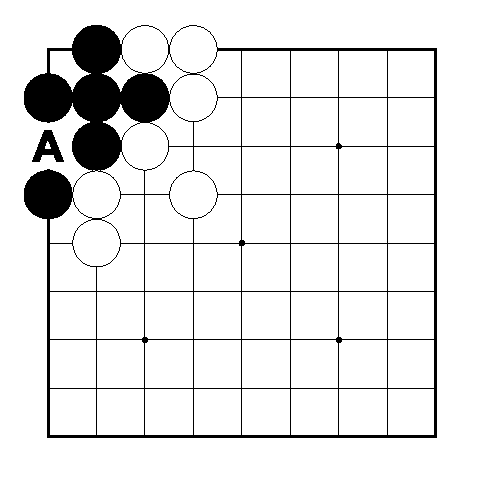
\includegraphics[width=1\textwidth]{8 - False Eyes - Dia 1}
        \caption*{\emph{Dia.\@~1}}
    \end{subfigure}
    \hspace{1cm}
    \begin{subfigure}[t]{.31\textwidth}
        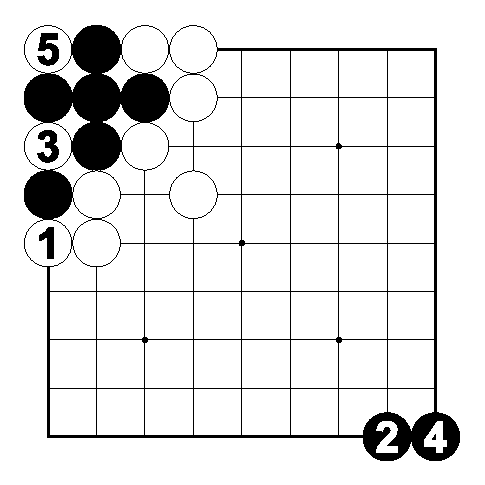
\includegraphics[width=1\textwidth]{8 - False Eyes - Dia 2}
        \caption*{\emph{Dia.\@~2. Preto 2 e 4 passam}}
    \end{subfigure}
\end{figure}

\emph{Dia.\@~2.} Teoricamente, no final da partida, Branco poderá capturar Preto com 1 a 5. Jogadores experientesnão jogariam tais movimentos, eles reconheceriam tal grupo como morto.

\pagebreak

\emph{Dia.\@~3.} Esse grupo preto não está morto ainda, mas Branco pode matá-lo.

\begin{figure}[h!]
    \centering
    \begin{subfigure}[t]{.31\textwidth}
        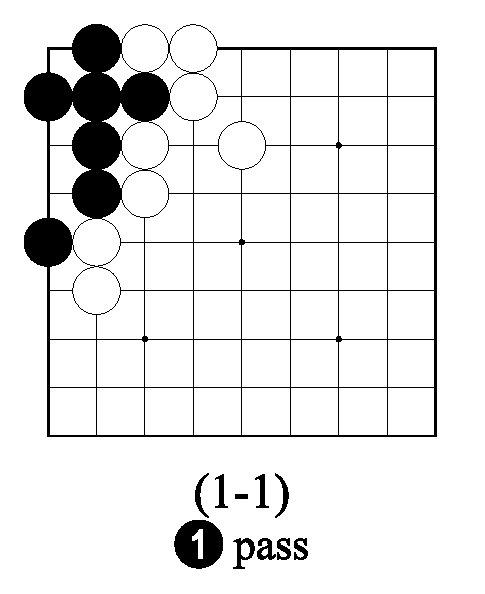
\includegraphics[width=1\textwidth]{8 - False Eyes - Dia 3}
        \caption*{\emph{Dia.\@~3}}
    \end{subfigure}
    \hfill
    \begin{subfigure}[t]{.31\textwidth}
        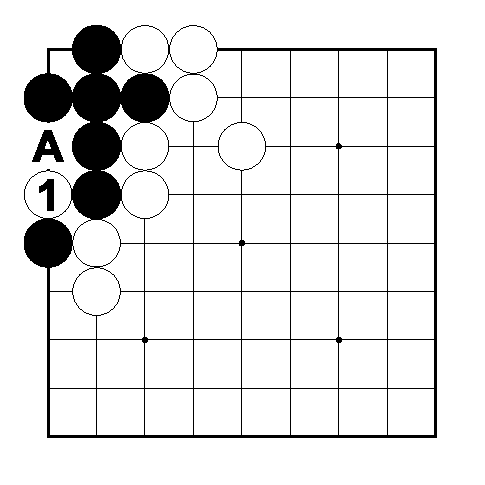
\includegraphics[width=1\textwidth]{8 - False Eyes - Dia 4}
        \caption*{\emph{Dia.\@~4}}
    \end{subfigure}
    \hfill
    \begin{subfigure}[t]{.31\textwidth}
        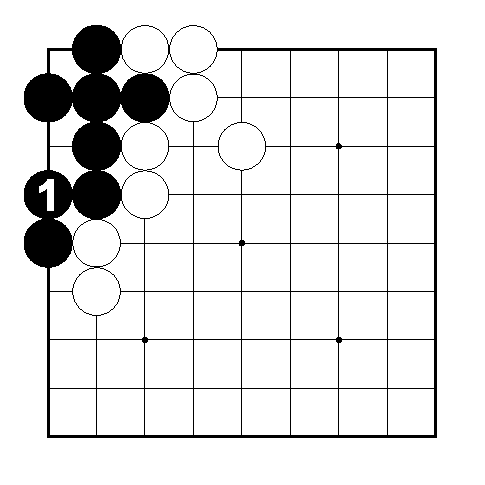
\includegraphics[width=1\textwidth]{8 - False Eyes - Dia 5}
        \caption*{\emph{Dia.\@~5}}
    \end{subfigure}
\end{figure}

\emph{Dia.\@~4.} Branco sacrifica uma pedra com 1, fazendo com que o segundo olho preto se torne falso. Se Preto capturar essa pedra com \textbf{A}, ele acabará com uma posição que é essencialmente idêntica ao \emph{Dia.\@~1}.

\emph{Dia.\@~5.} Para fazer dois olhos, Preto precisa conectar em 1. O grupo preto não poderá, então, mais ser morto.

\subsection{Exemplo 1}

O grupo preto no \emph{Dia.\@~1} está instável. Ele viverá ou morrerá, dependendo de qual será o próximo movimento.

\begin{figure}[h!]
    \centering
    \begin{subfigure}[t]{.31\textwidth}
        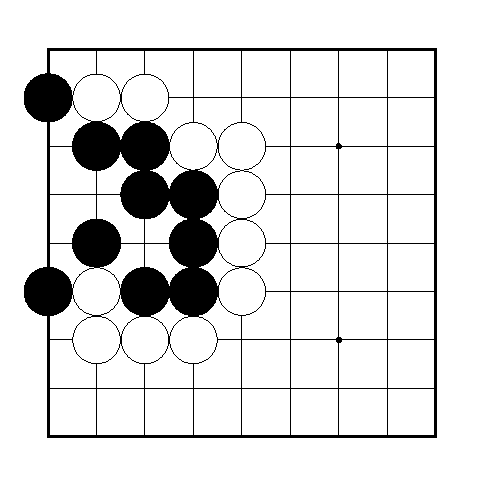
\includegraphics[width=1\textwidth]{8 - False Eyes - Example 1 - Dia 1}
        \caption*{\emph{Dia.\@~1. Instável}}
    \end{subfigure}
    \hspace{1cm}
    \begin{subfigure}[t]{.31\textwidth}
        \includegraphics[width=1\textwidth]{8 - False Eyes - Example 1 - Dia 2}
        \caption*{\emph{Dia.\@~2. Morto}}
    \end{subfigure}
\end{figure}

Se Branco jogar primeiro, ele matará Preto com a colocação de 1 no \emph{Dia.\@~2}. Se Preto conectar com 2, Branco toma o ponto-chave de 3. Após a captura preta com 4\ldots

Branco sacrifica uma pedra com 5 no \emph{Dia.\@~3}, criando um olho falso naquele ponto. Preto não consegue mais fazer um segundo olho, portanto seu grupo está morto.

Se Preto jogar primeiro, ele poderá fazer um segundo olhopara seu grupo pela conexão de 1 no \emph{Dia.\@~4}. Se Branco \textbf{A}, Preto captura em \textbf{B} e obtém seus dois olhos.

\subsection{Exemplo 2}

O grupo preto no \emph{Dia.\@~1} está instável, incompleto. Ele viverá ou morrerá baseado no próximo movimento.

Se Branco jogar primeiro, ele poderá matar o grupo preto com o sacrifício de 1 no \emph{Dia.\@~2}. O ponto 1 agora é um olho falso. Capturar com 2 não ajuda Preto a criar um olho. Seu grupo está morto a partir daí.

O ponto \textbf{A} no \emph{Dia.\@~3} é um olho falso. Apesar de que Branco não precisa jogar lá, ele pode forçar Preto a jogar naquele ponto com o atari em \textbf{B}, se desafiado a demonstrar que o grupo Preto está morto.

Se Preto jogar primeiro, ele pode fazer um segundo olho para seu grupo conectando em 1 no \emph{Dia.\@~4}.

\subsection{Exemplo 3}

O grupo preto no \emph{Dia.\@~1} está incompleto. Vida ou morte dependem da próxima jogada.

Se Branco jogar primeiro, ele poderá jogar 1 no \emph{Dia 2} e transformar o olho em \textbf{A} em um olho falso. Preto está morto.

Se for turno preto, ele pode tornar o ponto \textbf{A} no \emph{Dia.\@~3} em um olho verdadeiro conectando em 1. 

\section{Espaço de Olho e Forma de Olho}

Quando um grupo cerca um espaço contíguo aberto de vários pontos, a questão de se esse espaço será suficientemente grande para assegurar dois olhos surge.

\emph{Dia.\@~1.} O grupo preto possui um espaço de três intersecções como olho, e seu status é instável.

\emph{Dia.\@~2.} Se Preto jogar 1, ele está vivo, pois possui dois olhos separados.

\emph{Dia.\@~3.} Porém, se Branco jogar 1, Preto está morto.

\emph{Dias. 4 e 5.} Os movimentos até Branco 11 nesses dois diagramas provam que o grupo Preto está morto. Branco simplesmente preenche todas as liberdades pretas mostradas. Preto não tem como se defender.

Aqui seguem mais alguns exemplos.

\emph{Dia.\@~6.} O grupo preto possui um olho de quatro espaços, e está vivo já.

\emph{Dia.\@~7.} Se Branco jogar em 1, Preto joga 2 e, novamente, ele está vivo com dois olhos separados.

\emph{Dia.\@~8.} Similarmente, se Branco jogar 1, Preto jogará 2 e, novamente, ele estará vivo com dois olhos separados.

\emph{Dia.\@~9.} Após Branco 1, Preto não pode passar ou ignorar o movimento branco. Branco continuará com 3 e Preto morrerá.

\emph{Dia.\@~10.} Branco pode demonstrar que Preto está morto jogando 5 a 9. Depois da captura por Preto em 10\ldots

\emph{Dia.\@~11.} Branco joga em 11, e a situação se torna clara: Preto não possui dois olhos.

\emph{Dia.\@~12.} O grupo preto está vivo ou morto, dependendo de quem for a vez.

\emph{Dia.\@~13.} Se for turno branco, e ele jogar em 1, o grupo preto está morto.

\emph{Dia.\@~14.} Se for turno preto, ele pode fazer três olhos jogando em 1.

\emph{Dia.\@~15.} O grupo preto é um quadrado de quatro espaços, e está morto já.

\emph{Dia.\@~16.} Mesmo se Preto jogar primeiro, tudo que ele pode fazer é jogar em 1 (ou qualquer outro ponto simétrico) e ameaçar fazer dois olhos jogando em 2. No entanto, Branco pode jogar 2 primeiro, e Preto é deixado sem uma resposta. Se ele jogar qualquer um entre \textbf{A} ou \textbf{B}, ele coloca todo seu grupo em atari.

\emph{Dia.\@~17.} Se Branco for desafiado a provar que o grupo Preto está morto, tudo que ele precisa fazer é jogar o atari em 4. Se Preto 5 capturar, Branco 6 joga novamente em 4, e todo o grupo preto inevitavelmente será capturado.

\emph{Dia.\@~18.} O grupo preto está vivo ou morto, dependendo de quem for o turno.

\emph{Dia.\@~19.} Se Branco jogar primeiro, ele pode matar Preto com 1. Esse movimento põe as cinco pedras pretas em atari. Se Preto conectar em \textbf{A}, todas as pedras estarão em atari. Após Branco 1, o grupo preto está morto, e a posição já está sedimentada.

\emph{Dia.\@~20.} Se for turno preto, ele pode viver jogando no ponto-chave de 1. Preto está vivo em seki. A posição fica como está. No final da partida, as três pedras brancas permanecerão no tabuleiro, e tanto Preto quanto Branco receberão zero pontos de território nesta região.

\emph{Dia.\@~21.} Se Branco resistir respondendo Preto 1, no \emph{Dia.\@~20}, com 2, Preto captura as quatro pedras brancas com 3.

\emph{Dia.\@~22.} Esse é o resultado da captura das pedras brancas no \emph{Dia.\@~21}. Preto está vivo com quatro pontos de território mais quatro pedras capturadas. Se Branco \textbf{A}, Preto ganha dois olhos jogando em \textbf{B}. Se Branco \textbf{B}, Preto \textbf{A}. Resistir, como no \emph{Dia.\@~21}, é uma perda de oito pontos para Branco.

\emph{Dia.\@~23.} O grupo preto possui um olho de cinco espaços. Ele está vivo ou morto, dependendo de quem for o turno.

\emph{dia. 24.} Depois de Branco 1, não mais nenhuma maneira com que Preto possa fazer dois olhos. Se necessário realmente capturar o grupo, Branco pode colocá-lo sob atari ocupando as intersecções marcadas com \textbf{X}. Se Preto, então, capturar com \textbf{A}, Preto acaba com um olho de quatro espaços, que é a mesma posição do \emph{Dia.\@~15}, onde mostramos que o grupo Preto está morto já.

\emph{Dia.\@~25.} Se for turno preto, ele poderá fazer dois olhos jogando no ponto-chave de 1.

O tópico de espaço de olho é minuciosamente contemplado no livro \emph{The Basics of Life and Death}~\cite{zeijst_bozulich_basics_of_life_and_death}, publicado pela Kiseido.
    \chapter{Estratégia de Go com Compensação}\label{chap:estrat_comp}

Depois de ter estudado, nos capítulos anteriores deste livro, e ter jogado algumas partidas em tabuleiros menores, você já adquiriu um conhecimento básico das regras e táticas básicas, então já está bem encaminhado para se tornar um jogador de Go. O próximo tópico que você precisará aprender é o de princípios básicos de estratégia no jogo. A forma mais segura de aprender tais princípios é estudando Go com pedras de compensação. Isso significa procurar por oponentes mais fortes e, com prazer, tomar grandes compensações contra eles. Jogar Go com compensação vai lhe ensinar como utilizar suas pedras de vantagem para ganhar influência no centro. Apesar de que o objetivo do Go é assegurar mais território do que o adversário, é influência que, lenta mas certamente, se torna território.

A maior compensação que existe tradicionalmente é a de nove pedras. É na verdade uma compensação enorme, equivalente a uma rainha no xadrez. Ainda assim, como iniciante, levará um bom tempo antes que você possa derrotar até mesmo um 1 dan razoavelmente forte, com essa compensação.

Encontrar oponentes hoje em dia é fácil. Há um excelente site chamado KGS (\href{https://www.gokgs.com}{\path{gokgs.com}})~\cite{kgs} onde você pode jogar online gratuitamente e, ainda, achar oponentes desde a sua própria força até a de profissionais.

Nós nos restringiremos esta discussão à compensação de nove pedras e somente estudaremos alguns padrões básicos que surgem com frequência neste nível de compensação.

\bigskip

Branco geralmente começa se aproximando uma das pedras de compensação no canto com 1 no \emph{Dia.\@~1}. A resposta preta mais forte é contatar com o movimento diagonal de 2. Branco responde, na maioria das vezes, estendendo em 3, e Preto pode delimitar seu território no topo com 4.

A razão pela qual a troca de Preto 2 por Branco 3 é boa para Preto é que a pedra marcada está atacando as duas pedras brancas. Em outras palavras, ela está atuando como uma pinça em conjuntura com as três pedras pretas no topo.

Idealmente, Branco gostaria de estender tão longe quanto \textbf{A}, mas a pedra marcada está no caminho. (Veja os princípios de extensão na página 36.)

Para compreender a razão que faz com que Preto primeiro contate em 2, suponhamos que Preto omita tal jogada e simplesmente estenda para 2 no \emph{Dia.\@~2}. Branco poderia, então, deslizar a 3, Preto defende com a diagonal de 4, e Branco estende para 5. Comparado à posição em \emph{Dia.\@~1}, as pedras brancas estão muito mais resilientes. Elas estão tomando território e estão muito mais avançadas no critério de fazer dois olhos e viver.

\section{A Estratégia Branca de Chapelação}

Após Preto 4 no \emph{Dia.\@~1}, Branco talvez faça a aproximação de dois espaços contra a pedra preta no canto inferior direito com 5 no \emph{Dia.\@~3}. Preto 6, delimitando o território no lado inferior, é um bom movimento e a resposta padrão. Branco poderá talvez, então, chapelar a pedra preta no lado direito com 7, ameaçando ostensivamente fazer território ele mesmo. Na realidade, ele está na esperança de atiçar Preto para uma briga, em que a habilidade de luta branca, sendo este o jogador mais forte, será muito superior à preta.

Como Preto deveria responder?

A melhor estratégia é, resolutamente, escapar ao centro com a pedra marcada, jogando a diagonal de 8.

Branco tenta mander Preto confinado ao lado direito com 9 a 11 no \emph{Dia.\@~4}, mas, depois de 12, Branco precisa cortar em 13 para eliminar a conexão preta ali. Preto então faz atari com 14 a 16, e suas pedras agora escaparam. Branco faz atari com 17, e assegura sua posição com 19 --- Branco talvez também jogue em \textbf{A}. Após 20, Preto já quase assegurou a maior parte do território na parte baixa do lado direito. Exceto pela captura de 12, Branco não possui nenhum território.

\bigskip

Outra estratégia que Preto pode empregar contra a estratégia branca de chapelação é a de ceder território no lado direito. Por exemplo, Preto pode começar por contra-chapelar em 8 no \emph{Dia.\@~5}, ameaçando de se conectar com a pedra marcada. Branco defende em 9. Preto agora pula a 10, induzindo Preto a defender em 11. Preto agora expande seu território no canto com 12, ameaçando reduzir o território e expandir o seu ainda mais, através do deslize em \textbf{A}.

Branco provavelmente defenderá com 13 no \emph{Dia.\@~6}. Preto continuará ameaçando reduzir o território branco com 14 a 16, enquanto expande seus cantos direitos superior e inferior. A continuação até 25 ainda também termina em sente.

Ao avaliar essa posição, podemos perceber que Branco assegurou aproximadamente vinte e cinco pontos em um território já fortemente delimitado. Entretanto, os cantos Pretos são estimados em mais de quarenta pontos. Adicionalmente, Preto terminou em sente, então ele ainda pôde reforçar sua posição no canto superior esquerdo com 26. Esse movimento tornará uma invasão branca nessa região exponencialmente mais difícil.

\section{Evitando a Estratégia Branca de Chapelação}

Ao invés de responder Branco 5 com 6 no \emph{Dia.\@~3}, uma jogada mais positiva é o pulo até 6 no \emph{Dia.\@~7}. Há duas razões por que esse é um bom movimento.

Primeiramente, Preto 6 cria uma barreira entre a pedra em 5 e a pedra branca marcada acima, assim mantendo os grupos separados. Branco agora está fragmentado em dois grupos sob ataque.

Em segundo lugar, Preto 6 se certifica de que a pedra marcada poderá se conectar à sua pedra no centro.

É esperado que Branco faça uma dupla-aproximação contra a pedra de compensação no canto inferior direito. Preto deveria então responder com o movimento diagonal em 8. Esse movimento segue o mesmo princípio de Preto 6: ele mantém as pedras brancas de 5 a 7 separadas e oferece acesso ao centro para a pedra 4-4, fazendo com que seja mais fácil conectá-la a seus aliados no exterior.

Há várias maneiras de Branco responder a Preto 8. Ele talvez ignore tal movimento e jogue em um lugar totalmente diferente; ele talvez, também, construa uma posição no lado inferior; ou ele talvez invada o canto como no \emph{Dia.\@~8} da próxima página.

\section{Construindo uma Armação de Território em Formato de Caixa}

Branco geralmente responde Preto 8 invadindo o canto com 9 no \emph{Dia.\@~8}, mas isso não terá um bom resultado para ele. Preto bloqueia com 10, e Branco cria um grupo vivo no canto com os movimentos até 19. Porém, com 20, Preto consegue uma parede densa virada para o centro, constituindo uma armação de território em formato de caixa jundo com as pedras marcadas. Além disso, as duas pedras brancas marcadas são basicamente inúteis à sombra da parede preta.

Branco talvez tente deslizar  para 9 no \emph{Dia.\@~9}. Novamente, Preto almeja o centro ao jogar 10. Branco cria um grupo vivo com 11 e 13, mas Preto mapeia uma grande armação de território em formato de caixa com 12 e 14. Com jogo claro e limpo, isso deveria gerar mais de 40 pontos garantidos de território para Preto.

Branco poderia estender para 9, esperando parar o avanço preto rumo à grande armação. Preto ancorará suas pedras no canto com 10. Se Branco pular para 11, Preto mantém Branco separado em dois. Branco terá muitas dificuldades vivendo com ambos os grupos.

\section{Expanda o Seu Território Atacando}

Depois da troca de 1 por Preto 4, Branco talvez tente criar uma base para suas pedras estendendo até 5 (ou \textbf{A}) em \emph{Dia.\@~11}. A resposta preta mais forte é fazer o ``pilar de ferro" com 6. Essa jogada previne a base branca no contato em 6 ou o deslize em \textbf{B}. Esse pilar de ferro também reforça a formação de caixa delineada pelas pedras marcadas.

Branco não possui espaço para expansão no topo, então ele se expande ao centro. Preto mantém a pressão nas pedras brancas pulando a 8 e continuando a expandir e fortalecer sua armação no lado esquerdo.

Já que Preto reforçou sua formação de caixa no canto superior esquerdo com as pedras marcadas, Branco estará em desvantagem se ali invadir. Portanto, ele talvez opte por jogar em uma parte do tabuleiro onde Preto possui menos pedras, esperando que qualquer posição que ele construa ali negue a influência preta da armação no canto superior esquerdo. No entanto, se ele tentar invadir essa área com 9 no \emph{Dia.\@~12}, Preto simplesmente enclausurará o canto com 10. Pular para Branco 11 é uma resposta razoável, mas Preto delimita o território no canto topo com 12. Jogando-se corretamente, Preto pode contar com pelo menos 25 pontos nessa região se tornando território seguro. No meio-tempo, Branco assegurou quase nenhum território e ele ainda possui duas pedras no lado esquerdo que precisam se estabilizar. 

Se Branco se aproximar do outro lado com 9 no \emph{Dia.\@~13}, Preto irá novamente enclausurar o canto com 10, dessa maneira assegurando o território no lado esquerdo com 12, após o pulo branco até 11. Este resultado é ainda pior para Branco do que \emph{Dia.\@~12}, visto que suas pedras de 9 a 11 estão espremidas  entre duas posições fortes pretas. Será uma tarefa árdua se estabilizar com tal grupo branco.

Por fim, Branco talvez invada diretamente o canto com 9 no \emph{Dia.\@~14}. Ele certamente pode criar um grupo vivo com quase dez pontos de território, mas à concessão de quase 30 pontos de potencial território, que muito provavelmente o será, com jogadas corretas.

\bigskip

Este capítulo é somente uma breve introdução à estratégia de compensação, em particular, a de nove pedras. Para uma discussão mais detalhada dessas posições, referenciam-se ao leitor \emph{Handicap Go Strategy and the Sanrensei Opening}~\cite{zeijst_bozulich_handicap_sanrensei}, disponível em forma impressa pela Kiseido (veja o \autoref{ap:pt} de catálogo de livros); ou, em sistemas iOS, o aplicativo SmartGo. Esse livro também é uma boa introdução a Go com compensação, assim como à abertura sanrensei, que é uma abertura de partidas em igualdade. Para um livro ainda mais detalhado sobre esse tópico, veja \emph{Handicap Go}~\cite{nagahara_bozulich_handicap_go}, também publicado pela Kiseido e disponível no aplicativo \href{apps.apple.com/us/app/smartgo-player/id314506629}{SmartGo}~\cite{smartgo}.
    \chapter{Níveis e Compensações}

O sistema de nivelamento amador utilizado no Go funciona da seguinte maneira. Jogadores iniciantes recebem automaticamente o nível de 35 kyu e, conforme aprendem técnicas básicas do jogo, eles rapidamente avançam a escada kyu até chegar a algo entre, aproximadamente 20 a 10 kyu. Essa melhora rápida presume, claro, que se estude e jogue algumas vezes na semana por alguns meses. De 10 a 1 kyu, o progresso é usualmente muito mais devagar. Assim que um jogador amador se torna um expert, ele recebe o nível de 1 dan (\emph{shodan} em japonês), ou de uma organização ou por simplesmente medir sua força contra outros jogadores de força dan. Níveis amadores dan vão até 7 dan em geral. Níveis profissionais vão de 1 a 9 dan, mas eles estão em uma escala diferente, portanto não possuem nenhum nível correspondente em níveis amadores. Um profissional 1 dan deveria estar apto a dar perto de três pedras de compensação a um amador de nível 5 dan, e ainda ter pelo menos 50\% de chance de vitória. O sistema de compensação no Go oferece ao jogador mais fraco uma chance realística de vitória quando se joga com alguém mais forte, dado que a compensação esteja correta, claro.

Jogadores de força igual geralmente utilizam um método chamado de \emph{nigiri} para determinar quem tomará branco ou preto. Quando o nigiri é utilizado, um dos jogadores toma uma quantidade arbitrária de pedras brancas enquanto que o jogador preto escolhe uma ou duas pedras, essencialmente uma variante do jogo de par-ou-ímpar. Então ambas as respectivas pedras escolhidas são postas em cima do tabuleiro. Se o número de pedras brancas corresponder à escolha de par ou ímpar preta, então cada jogador procede com suas cores como estão, senão os jogadores trocam suas cores. Dali em diante, o jogo procede normalmente. Porém, caso um dos jogadores comece a ganhar consistentemente, a compensação deve mudar.

O jogador com as pedras pretas sempre possui o primeiro movimento, então ele possui uma vantagem crítica. Essa vantagem é estimada como de valia de 6 pontos. Portanto, quando de jogadores de força similar, o jogador com pedras pretas dá ao de pedras brancas seis prisioneiros no início da partida, como adiantamento. Adicionalmente, se o resultado da partida for empate, Branco vence. Esse total de prisioneiros é referenciado como \emph{komi}, e dizemos algo como ``Branco recebe um komi de 6.5 pontos".

Quando jogadores de diferentes níveis jogam uma partida, o jogador mais forte sempre toma as pedras brancas, e a compensação é determinada pela diferença de nível entre eles. Por exemplo, se um jogador for 1 kyu, e o outro, 2 kyu, então o jogador 2 kyu não recebe nenhuma pedra de compensação. Em seu lugar, ele joga como preto sem nenhum komi, fazendo o primeiro movimento.

Quando um 1 kyu joga contra um 3 kyu, o 3 kyu recebe uma compensação de duas pedras; quando um 1 kyu joga contra um 5 kyu, o 5 kyu recebe uma compensação de quatro pedras, etc., até a compensação de nove pedras, que é em geral a maior dada.

O mesmo sistema de compensação é utilizado para jogadores de nível dan também. A princípio, é possível determinar sua força no Go jogando contra jogadores de níveis já bem estabelecidos. No entanto, até um amador se tornar aproximadamente 5 dan, sua força pode oscilar fortemente. Por fim, apesar de que o sistema de nível do Go é virtualmente o mesmo ao redor do mundo, o valor dado a tais níveis pode variar de lugar para lugar.

Assim que a compensação para o jogador mais fraco for estabelecida, ele coloca pedras de compensação no tabuleiro na ordem exibida nos diagramas abaixo (\emph{Dias. 15 a 17}). Branco então faz o primeiro movimento real da partida, e ambos os jogadores se alternam. Por exemplo, se a compensação for de três pedras, Preto posicionaria as pedras 1, 2 e 3 (a ordem tradicional) no \emph{Dia.\@~15}, e Branco faria o primeiro movimento real da partida.

\begin{figure}[h!]
    \centering
    \begin{subfigure}[t]{.45\textwidth}
        \includegraphics[width=1\textwidth]{10 - Dia 15}
        \caption*{\emph{Dia.\@~15}}
    \end{subfigure}
    \hspace{1cm}
    \begin{subfigure}[t]{.45\textwidth}
        \includegraphics[width=1\textwidth]{10 - Dia 16}
        \caption*{\emph{Dia.\@~16}}
    \end{subfigure}
\end{figure}

\begin{figure}[h!]
    \centering
    \begin{subfigure}[t]{.45\textwidth}
        \includegraphics[width=1\textwidth]{10 - Dia 17}
        \caption*{\emph{Dia.\@~17}}
    \end{subfigure}
\end{figure}

Seguindo estritamente as regras (\emph{Regra 4} em particular, no \autoref{chap:regras}), o que realmente está acontecendo é que, após Preto posicionar 1, Branco passa. Preto então coloca a pedra 2 (na realidade, o terceiro movimento), e, novamente, Branco passa. Preto joga 3 (movimento 4), mas Branco não passa e faz seu primeiro movimento, iniciando realmente a partida.

De acordo com a \emph{Regra 3}, um jogador pode jogar em qualquer ponto que quiser, então ele poderia jogar pedras de compensação em qualquer intersecção. É possível jogar assim, desde que negociado entre os jogadores. Porém, de um ponto de vista pedagógico, nós recomendamos seguir a maneira tradicional de se jogar Go, pois ela vai lhe ensinar como jogar com pedras no 4-4 e criar posições fortes e densas.
    \chapter{Movimentos de Fim de Jogo}

A posição no \emph{Dia.\@~1} abaixo é a mesma que no \emph{Dia.\@~6} do \autoref{chap:estrat_comp} após Branco ter jogado 13 (a pedra marcada). Quando Preto desce para 1 (14 no \emph{Dia.\@~6} do \autoref{chap:estrat_comp}), Branco não deveria jogar em outro lugar, com 2 por exemplo, já que Preto invadirá com 3, e Branco não conseguirá defender seu território.

\begin{figure}[h!]
    \centering
    \begin{subfigure}[t]{.475\textwidth}
        \includegraphics[width=1\textwidth]{11 - Dia 1}
        \captionsetup{justification=centering}
        \caption*{\emph{Dia.\@~1}}
    \end{subfigure}
    \hfill
    \begin{subfigure}[t]{.475\textwidth}
        \includegraphics[width=1\textwidth]{11 - Dia 2}
        \captionsetup{justification=centering}
        \caption*{\emph{Dia.\@~2}}
    \end{subfigure}
\end{figure}

O melhor que ele pode fazer, no caso da invasão, é empurrar com 4 no \emph{Dia.\@~2} e pular para 6. Porém, Preto pode reduzir Branco rastejando com 7 a 9. Após os movimentos até 13, o território branco basicamente desapareceu. Branco investiu movimentos demais nesta área para deixar que isso ocorra.

\pagebreak

\begin{wrapfigure}{r}{60mm}
    \vspace{-20pt}
    \begin{center}
        \includegraphics[width=.5\textwidth]{11 - Dia 3}
        \captionsetup{justification=centering}
        \caption*{\emph{Dia.\@~3}}
    \end{center}
    \vspace{-31pt}
\end{wrapfigure}

Sendo assim, quando Preto desce para 1 no \emph{Dia.\@~3}, Branco não possui nenhuma outra escolha senão defender com 2. Quando Preto desce para 3, ele precisa bloquear com 4 também.

Movimentos como Preto 1 e 3 são geralmente jogados no final do meio de jogo quando o território de cada lado já foi essencialmente determinado. Eles são utilizados para expandir territórios ao mesmo tempo que diminuem os do adversário. Em seguida\ldots

\pagebreak

Preto joga 5 e 7 no \emph{Dia.\@~4}, forçando Preto a defender com 6 e 8. Ele continua com o mesmo tipo de movimento na parte inferior do lado direito com 9 e 11, e Branco precisa defender com 12, terminando em \emph{gote}. Em outras palavras, Branco precisa fazer o último movimento defensivo.

\begin{figure}[h!]
    \centering
    \begin{subfigure}[t]{.475\textwidth}
        \includegraphics[width=1\textwidth]{11 - Dia 4}
        \captionsetup{justification=centering}
        \caption*{\emph{Dia.\@~4}}
    \end{subfigure}
    \hfill
    \begin{subfigure}[t]{.475\textwidth}
        \includegraphics[width=1\textwidth]{11 - Dia 5}
        \captionsetup{justification=centering}
        \caption*{\emph{Dia.\@~5}}
    \end{subfigure}
\end{figure}

Por que Branco 8 e 12 seriam necessários?

Depois de Branco 12 no \emph{Dia.\@~4}, Preto possui sente. Isto é, ele possui a iniciativa --- ele não precisa defender e pode jogar onde quiser. Nesta posição, ele talvez queira jogar em \textbf{A} ou \textbf{B} e conseguiu uma boa vantagem nesta parte do tabuleiro.

Se Branco omitir 8 no \emph{Dia.\@~4} e se aproximar da pedra preta no canto inferior esquerdo com 1 no \emph{Dia.\@~5}, Preto cortará com 2. Se Branco tentar escapar com 3, Preto faz atari de novo com 4 e, então, enreda com 6. As pedras brancas não conseguem fugir. Se Branco \textbf{A}, Preto faz atari em \textbf{B}; se Branco \textbf{C}, Preto \textbf{D}.

\pagebreak

\section{Cálculos de Fim de Jogo}

Restrinjamos nossa atenção ao lado direito do tabuleiro, assumindo que os outros territórios no tabuleiro já foram decididos. Qual é o valor dos movimentos Preto 5 e 7? E qual é o valor dos movimentos Preto 9 e 11?

\begin{figure}[h!]
    \centering
    \begin{subfigure}[t]{.3\textwidth}
        \includegraphics[width=1\textwidth]{11 - Dia 6}
        \captionsetup{justification=centering}
        \caption*{\emph{Dia.\@~6}}
    \end{subfigure}
    \hspace{1cm}
    \begin{subfigure}[t]{.3\textwidth}
        \includegraphics[width=1\textwidth]{11 - Dia 7}
        \captionsetup{justification=centering}
        \caption*{\emph{Dia.\@~7}}
    \end{subfigure}
\end{figure}

Supondo que Branco jogue como aqui, no \emph{Dia.\@~7} antes de Preto. Se Branco fizer 5, Preto precisa responder com 6. Branco conecta com 7 e Preto precisa defender com 8. Comparado a \emph{Dia.\@~6}, Branco ganhou dois pontos marcados com $\times$, e Preto perdeu dois pontos em 6 e 8. Isso é um ganho de quatro pontos para Branco\footnote{Em relação \emph{Dia. 4}, Branco possui 2 pontos a mais, e Preto, 2 a menos. No total, na comparação entre as duas sequências, temos uma diferença de $2 - (-2) = 2 + 2 = 4$.}.

Branco também termina com sente, então ele pode ainda jogar 9 e 11, forçando Preto a responder com 10 e 12. Comparado ao \emph{Dia.\@~6}, Branco ganha outros dois pontos, marcados com \(\increment\), e Preto perde dois pontos, 10 e 12. Novamente, Branco ganha quatro pontos.

Portanto, qual seja o lado que jogue seus movimentos primeiro, o ganho será de oito pontos.

\pagebreak

\begin{wrapfigure}{r}{60mm}
    \vspace{-20pt}
    \begin{center}
        \includegraphics[width=.5\textwidth]{11 - Dia 8}
        \captionsetup{justification=centering}
        \caption*{\emph{Dia.\@~8}}
    \end{center}
    \vspace{-25pt}
\end{wrapfigure}

No entanto, a posição no \emph{Dia.\@~1} surgiu na abertura, então Preto talvez não desça para 1. Em seu lugar, ele talvez reforce sua posição no canto superior esquerdo com 1 no \emph{Dia.\@~8}. Branco talvez pense que descer para 2 é um grande movimento, já que ameaça a invasão do canto Preto, mas Preto ignoraria  tal ameaça e asseguraria o canto superior esquerdo com 3 ou \textbf{A}.

Se Branco der continuidade à ameaça de invasão ao canto superior direito preto com 4 e 6, Preto assegurará o canto inferior esquerdo com 5 e 7. A invasão branca no canto superior direito é de aproximadamente 30 pontos, mas Preto 1 a 7 delimitam um território enorme à esquerda. É difícil estimar quão grande será esse território. Branco provavelmente conseguirá invadi-lo e criar um grupo vivo, mas Preto será capaz de garantir mais de 60 pontos no processo. Sendo assim, Preto fica feliz com a troca.

O que estamos querendo enfatizar é que movimentos como Preto 1 no \emph{Dia.\@~1} e Branco 2 no \emph{Dia.\@~8} são geralmente deixados mais para o fim de jogo. Na abertura, há sempre movimentos maiores a serem feitos. É claro que Preto 1 no \emph{Dia.\@~1} é uma grande ameaça, então, do ponto de vista do Branco, ele não pode ignorá-lo. Mas, do ponto de vista do Preto, ele pode facilmente se dar ao luxo de ignorar Branco 2 no \emph{Dia.\@~8}, já que há pontos maiores em disputa do que simplesmente defender o canto\footnote{A defesa do canto é muito mais um privilégio do Preto, pois somente Preto pode se dar ao luxo de não defender.}.

O fim de jogo é um aspecto importante do jogo a se dominar. A margem de vitória ou derrota é frequentemente muito pequena, e manobras hábeis de fim de jogo podem virar a partida a seu favor.

A Kiseido já publicou dois excelentes livros sobre esse assunto. Para uma introdução detalhada ao assunto, você deveria ler o \emph{The Endgame}~\cite{tomoko_bozulich_endgame}, Volume 6 da \emph{Elementary Go Series} da Kiseido. Outro livro recomendado é o \emph{Get Strong at the Endgame}~\cite{bozulich_endgame}, Volume 7 da \emph{Get Strong at Go Series} da Kiseido. Esse livro provê cálculos de fim de jogo para 101 posições básicas. Há também 120 problemas onde você deverá encontrar o tesuji de fim de jogo --- um movimento brilhante que cumpre um papel tático claro ---, que maximizará seu lucro. Ao final, há 70 problemas em tabuleiros 9\(\times\)9 e 13\(\times\)13, que lhe possiblitarão um teste de habilidade no fim de jogo.
    \chapter{Como Continuar os Estudos}



    \appendix
    \addtocontents{toc}{\vspace*{1cm}\noindent\textbf{Apêndice}\par}
    \chapter{Catálogo Kiseido em Inglês}\label{ap:en}

\emph{Books marked with an asterisk are also available on iOS via the Go Books~\cite{gobooks} app by SmartGo~\cite{smartgo}.}

\section{Introductory and General}

\begin{longtable}{l|p{50mm}|p{50mm}} 
    \hline
    \textbf{Code} & \textbf{Title} & \textbf{Author(s)} \\
    \hline \hline
    K50* & Go --- A Complete Introduction to the Game & Cho Chikun \\
    \hline
    K40 & The Go Player's Almanac 2001 & Richard Bozulich (editor) \\
    \hline
    K30 & Japanese Prints and the World of Go & William Pinckard and Kitagawa Akiko \\
    \hline
\end{longtable}


\section{Problem Books for Beginners}

\emph{Graded Go Problems for Beginners}, by Kano Yoshinori:

\begin{longtable}{c|c|l} 
    \hline
    \textbf{Code} & \textbf{Volume} & \textbf{Title} \\
    \hline \hline
    K46* & 1 & Introductory Problems (35-25 kyu) \\
    \hline
    K47* & 2 & Elementary Problems (25-20 kyu) \\
    \hline
    K48* & 3 & Intermediate Problems (20-15 kyu) \\
    \hline
    K49* & 4 & Advanced Problems (15-1 kyy) \\
    \hline
\end{longtable}


\section{Elementary Go Series}

For more than 30 years, the \emph{Elementary Go Series} has been the standard texts for Go players who want to get a firm grasp of the fundamentals of Go. Not only is the theory of Go elaborated on, the reader is also given problems to show how these theoretical concepts are applied in actual games.

\begin{longtable}{c|c|p{45mm}|p{45mm}} 
    \hline
    \textbf{Code} & \textbf{Volume} & \textbf{Title} &\textbf{Author(s)} \\
    \hline \hline
    K10* & 1 & In the Beginning --- The Opening in the Game of Go & Ishigure Ikuro \\
    \hline
    K11* & 2 & 38 Basic Josekis & Kosugi Kiyoshi and James Davies \\
    \hline
    K12* & 3 & Tesuji & James Davies \\
    \hline
    K13* & 4 & Life and Death & James Davies \\
    \hline
    K14* & 5 & Attack and Defense & Ishida Akira and James Davies \\
    \hline
    K15* & 6 & The Endgame & Ogawa Tomoko and James Davies \\
    \hline
    K16* & 7 & Handicap Go & Nagahara Yoshiaki and Richard Bozulich \\
    \hline
\end{longtable}

\section{Get Strong at Go Series}

A series of problem books covering every phase of the game, from the opening to the endgame. Each book contains 170 or more problems ranging in difficulty from elementary to advanced. Thus, they can be used by players ranging in strength from 20 kyu to dan-level. By studying Go in this problem format, you will not only learn basic principles as to why moves are made but also train yourself in thinking through and analyzing positions. You will encounter a great many of the same or similar patterns that will arise in your own games. We guarantee that diligent study of this entire series will lay the foundation for becoming a truly strong player.

\bigskip

\emph{All the books in this series are authored by Richard Bozulich.}

\begin{longtable}{l|c|l} 
    \hline
    \textbf{Code} & \textbf{Volume} & \textbf{Title} \\
    \hline \hline
    K51 & 1 & Get Strong at the Opening \\
    \hline
    K52 & 2 & Get Strong at Joseki I \\
    \hline
    K53 & 3 & Get Strong at Joseki II \\
    \hline
    K54 & 4 & Get Strong at Joseki III \\
    \hline
    K55 & 5 & Get Strong at Invading \\
    \hline
    K56 & 6 & Get Strong at Tesuji \\
    \hline
    K57* & 7 & Get Strong at the Endgame \\
    \hline
    K58* & 8 & Get Strong at Life and Death \\
    \hline
    K59* & 9 & Get Strong at Handicap Go \\
    \hline
    K60 & 10 & Get Strong at Attacking \\
    \hline
\end{longtable}

\section{Mastering the Basics}

A series of books, especially written for high-kyu players, for mastering the basic techniques of Go. Each book in this series consists of hundreds of problems designed to hammer home the fundamental concepts of Go theory and technique. A thorough and patient study of this series is the fastest way to advance through the kyu ranks.

\begin{longtable}{l|c|p{55mm}|p{35mm}} 
    \hline
    \textbf{Code} & \textbf{Volume} & \textbf{Title} & \textbf{Author(s)} \\
    \hline \hline
    K71* & 1 & 501 Opening Problems & Richard Bozulich and Rob van Zeijst \\
    \hline
    K72 & 2 & 1001 Life-and-Death Problems & Richard Bozulich \\
    \hline
    K73* & 3 & Making Good Shape & Rob van Zeijst and Richard Bozulich \\
    \hline
    K74* & 4 & 501 Tesuji Problems & Richard Bozulich \\
    \hline
    K75* & 5 & The Basics of Go Strategy & Richard Bozulich \\
    \hline
    K76* & 6 & All About Ko & Rob van Zeijst and Richard Bozulich \\
    \hline
    K77* & 7 & Attacking and Defending Moyos & Rob van Zeijst and Richard Bozulich \\
    \hline
    K78* & 8 & Fight Like a Pro --- The Secrets of Kiai & Rob van Zeijst and Richard Bozulich \\
    \hline
    K79* & 9 & An Encyclopedia of Go Principles & Richard Bozulich \\
    \hline
    K80 & 10 & Close Encounters with the Middle Game & Michiel Eijkhout \\
    \hline
\end{longtable}

\section{Elementary Books}

\begin{longtable}{l|p{55mm}|p{55mm}} 
    \hline
    \textbf{Code} & \textbf{Title} & \textbf{Author(s)} \\
    \hline \hline
    K02* & Basic Techniques of Go & Nagahara Yoshiaki and Haruyama Isamu \\
    \hline
    K28 & Lessons in the Fundamentals of Go & Kageyama Toshiro \\
    \hline
    K36 & Opening Theory Made Easy & Otake Hideo \\
    \hline
    K82* & Handicap Go Strategy and the Sanrensei Opening & Rob van Zeijst and Richard Bozulich \\
    \hline
    K83 & The Basic Principles of the Opening and Middle Game & Rob van Zeijst and Richard Bozulich \\
    \hline
    K84* & The Basics of Life and Death & Rob van Zeijst and Richard Bozulich \\
    \hline
    K85 & A Survey of Basic Tesujis & Richard Bozulich \\
    \hline
\end{longtable}

\section{Advanced Books}

From the \emph{Graded Go Problems for Dan Players} series:

\begin{longtable}{c|c|l} 
    \hline
    \textbf{Code} & \textbf{Volume} & \textbf{Title} \\
    \hline \hline
    K61 & 1 & 300 Life and Death Problems 5 kyu to 3 dan \\
    \hline
    K62 & 2 & 300 Tesuji Problems 5 kyu to 3 dan \\
    \hline
    K63 & 3 & 300 Joseki Problems 1 dan to 3 dan \\
    \hline
    K64 & 4 & 300 Life and Death Problems 4 dan to 7 dan \\
    \hline
    K65 & 5 & 300 Tesuji Problems 4 dan to 7 dan \\
    \hline
    K66 & 6 & 300 Joseki Problems 4 dan to 7 dan \\
    \hline
    K67 & 7 & Opening and Middle Game Problems 1 dan to 7 dan \\
    \hline
\end{longtable}

Other advanced books:

\begin{longtable}{l|p{55mm}|p{55mm}} 
    \hline
    \textbf{Code} & \textbf{Title} & \textbf{Author(s)} \\
    \hline \hline
    K81 & A Dictionary of Modern Fuseki: The Korean Style & Kim Song June \\
    \hline
    K29 & Reducing Territorial Frameworks & Fujisawa Shuko \\
    \hline
    K41 & The 21st Century Dictionary of Basic Joseki, Vol. 1 & Takao Shinji \\
    \hline
    K42 & The 21st Century Dictionary of Basic Joseki, Vol. 2 & Takao Shinji \\
    \hline
\end{longtable}

\section{Game Collections}

\begin{longtable}{l|p{55mm}|p{55mm}} 
    \hline
    \textbf{Code} & \textbf{Title} & \textbf{Author(s)} \\
    \hline \hline
    K01* & Invincible: The Games of Shusaku & John Power (editor and compiler) \\
    \hline
    K07 & The 1971 Honinbo Tournament & Iwamoto Kaoru \\
    \hline
    K91* & Modern Master Games, Vol. 1, The Dawn of Tournament Go & Rob van Zeijst and Richard Bozulich \\
    \hline
    K92 & Modern Master Games, Vol. 2, The 2014 Ten-Game Match between Gu Li and Lee Sedol, Part One: Games One to Five & Rob van Zeijst \\
    \hline
    K93 & Modern Master Games, Vol. 3, The 2014 Ten-Game Match between Gu Li and Lee Sedol, Part One: Games Six to Eight & Michael Redmond 9p and Rob van Zeijst \\
    \hline
    PP01 & Tournament Go 1992 & John Power (editor and compiler) \\
    \hline
\end{longtable}

\section{Go World}

\emph{Go World} was a quarterly magazine that covered the Japanese and international tournament scene. Analysis of games from tournaments and instructional articles for players of all levels.

A complete set of Go World from the first issue to issue \#129 is available on three DVDs from Kiseido Digital. To order, go to \href{https://www.kiseidodigital.com}{\path{kiseidodigital.com}}.

To order books and Go equipment, go to the online shop at Kiseido's website at \href{https://www.kiseido.com}{\path{kiseido.com}}.

\section{Direct from Japan}

Here is Kiseido's address in Japan:

\bigskip
\bigskip

\begin{tabular}{l}
    \hline
    Kiseido Publishing Company \\
    Kagawa 4-48-32 \\
    Chigasaki-shi \\
    Kanagawa-ken \\
    Japan 253-0082 \\
    FAX +81-467-81-0605 \\
    email: \href{mailto:kiseido@yk.rim.or.jp}{kiseido@yk.rim.or.jp} \\
    \href{https://www.kiseido.com}{kiseido.com} \\
    \hline
\end{tabular}
    \chapter{Catálogo Kiseido em Português}\label{ap:pt}

\emph{Note, porém, que, basicamente, nenhum dos livros abaixo foram traduzidos para o português. O catálogo abaixo é apenas uma tradução somente dos títulos em inglês.}

\bigskip
    \chapter{Jogue Go Online com o Kiseido Go Server (KGS)}

Jogue Go online gratuitamente através do Kiseido Go Server (KGS). Ele pode ser acessado através do site da Kiseido (\href{https://www.kiseido.com}{\path{kiseido.com}}~\cite{kiseido}), ou você pode ir diretamente ao \href{https://www.gokgs.com}{\path{gokgs.com}}~\cite{kgs}. Não há custo para se jogar partidas no servidor, e ele funciona com Linux/UNIX, Mac e Windows. A força dos jogadores vai desde iniciantes até profissionais 9 dans.

O KGS possui as seguintes funcionalidades:

\begin{enumerate}
    \item Edição de partidas online.
    \item O KGS é multilingual. Todas as mensagens que os jogadores digitam e enviam são feitas em Unicode, o que possibilita conversas em qualquer linguagem.
    \item Suporte primariamente de regras japonesas, mas também há como se utilizar regras chinesas, AGA (americanas) e neozelandesas.
    \item É possível jogar sem tempo limite, com um limite de tempo absoluto ou com vários sistemas de byo-yomi.
    \item Habilidade de salvar e exportar seus jogos gratuitamente, possibilitando revisões e estudos futuros.
    \item Sistema de nivelamento que possibilita, dentre outros, histórico de progresso. 
\end{enumerate}

Entre no KGS por \href{https://www.gokgs.com}{\path{gokgs.com}}~\cite{kgs}.

    \backmatter
    \bibliographystyle{unsrt}
    \bibliography{bibliografia}
\end{document}
%-------------------------------------------------------------------------------